\makeatletter
\tikzset{
  base/.is choice,
  base/top/.code={\let\vbox\vtop},
  base/bottom/.code={\def\pgfutil@minipage[t]{\minipage[b]}},
  % base/bottom/.code={}, % for plain TeX
}
\makeatother

%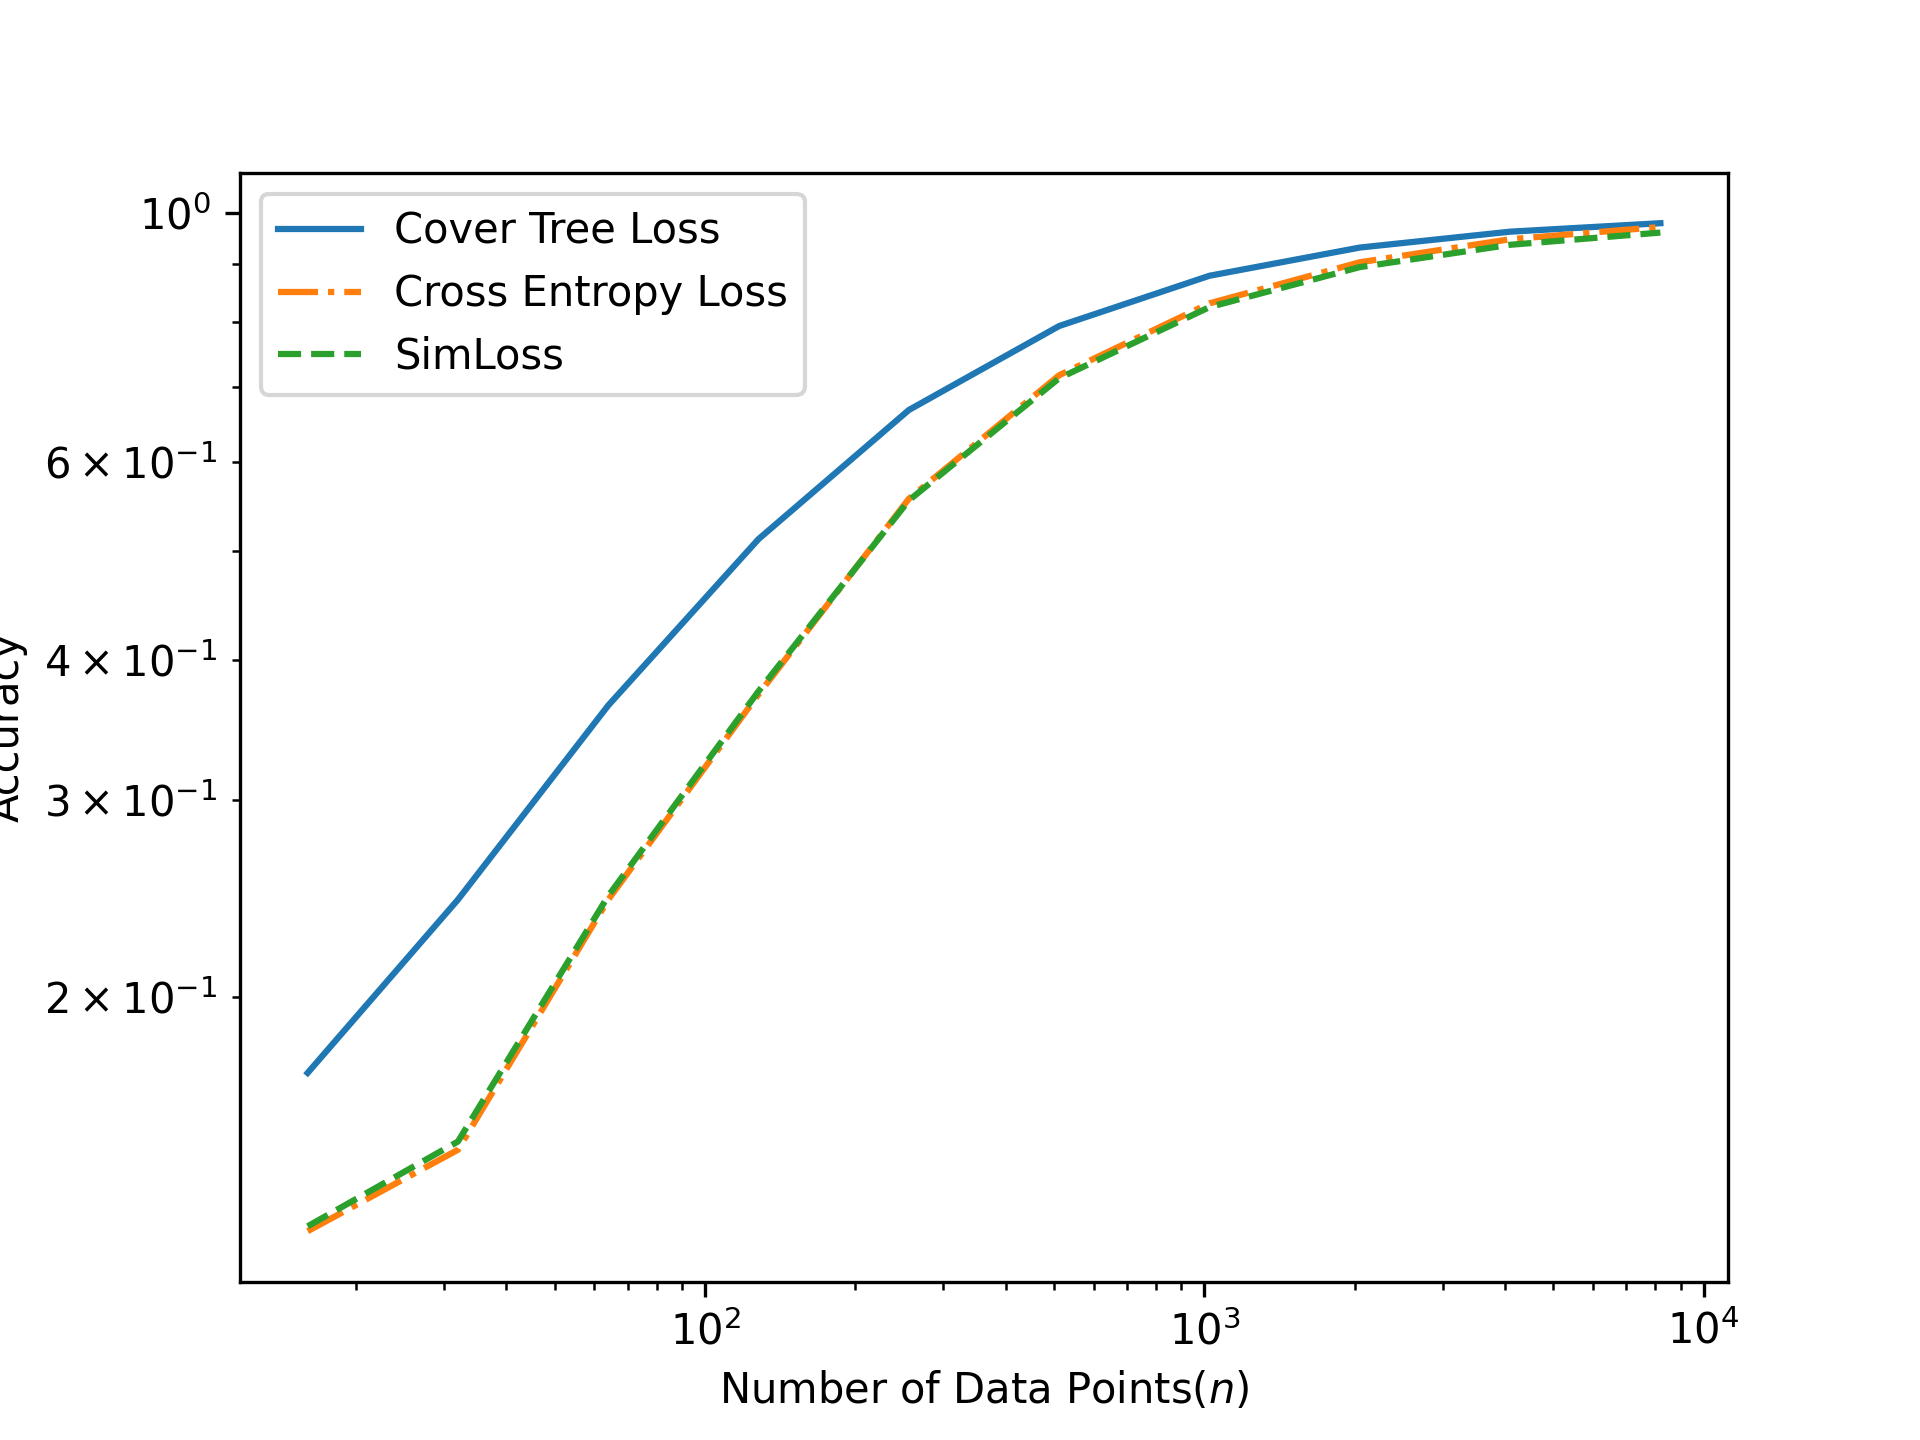
\includegraphics[width=0.48\columnwidth]{fig/images/accuracy_vs_n.png}
%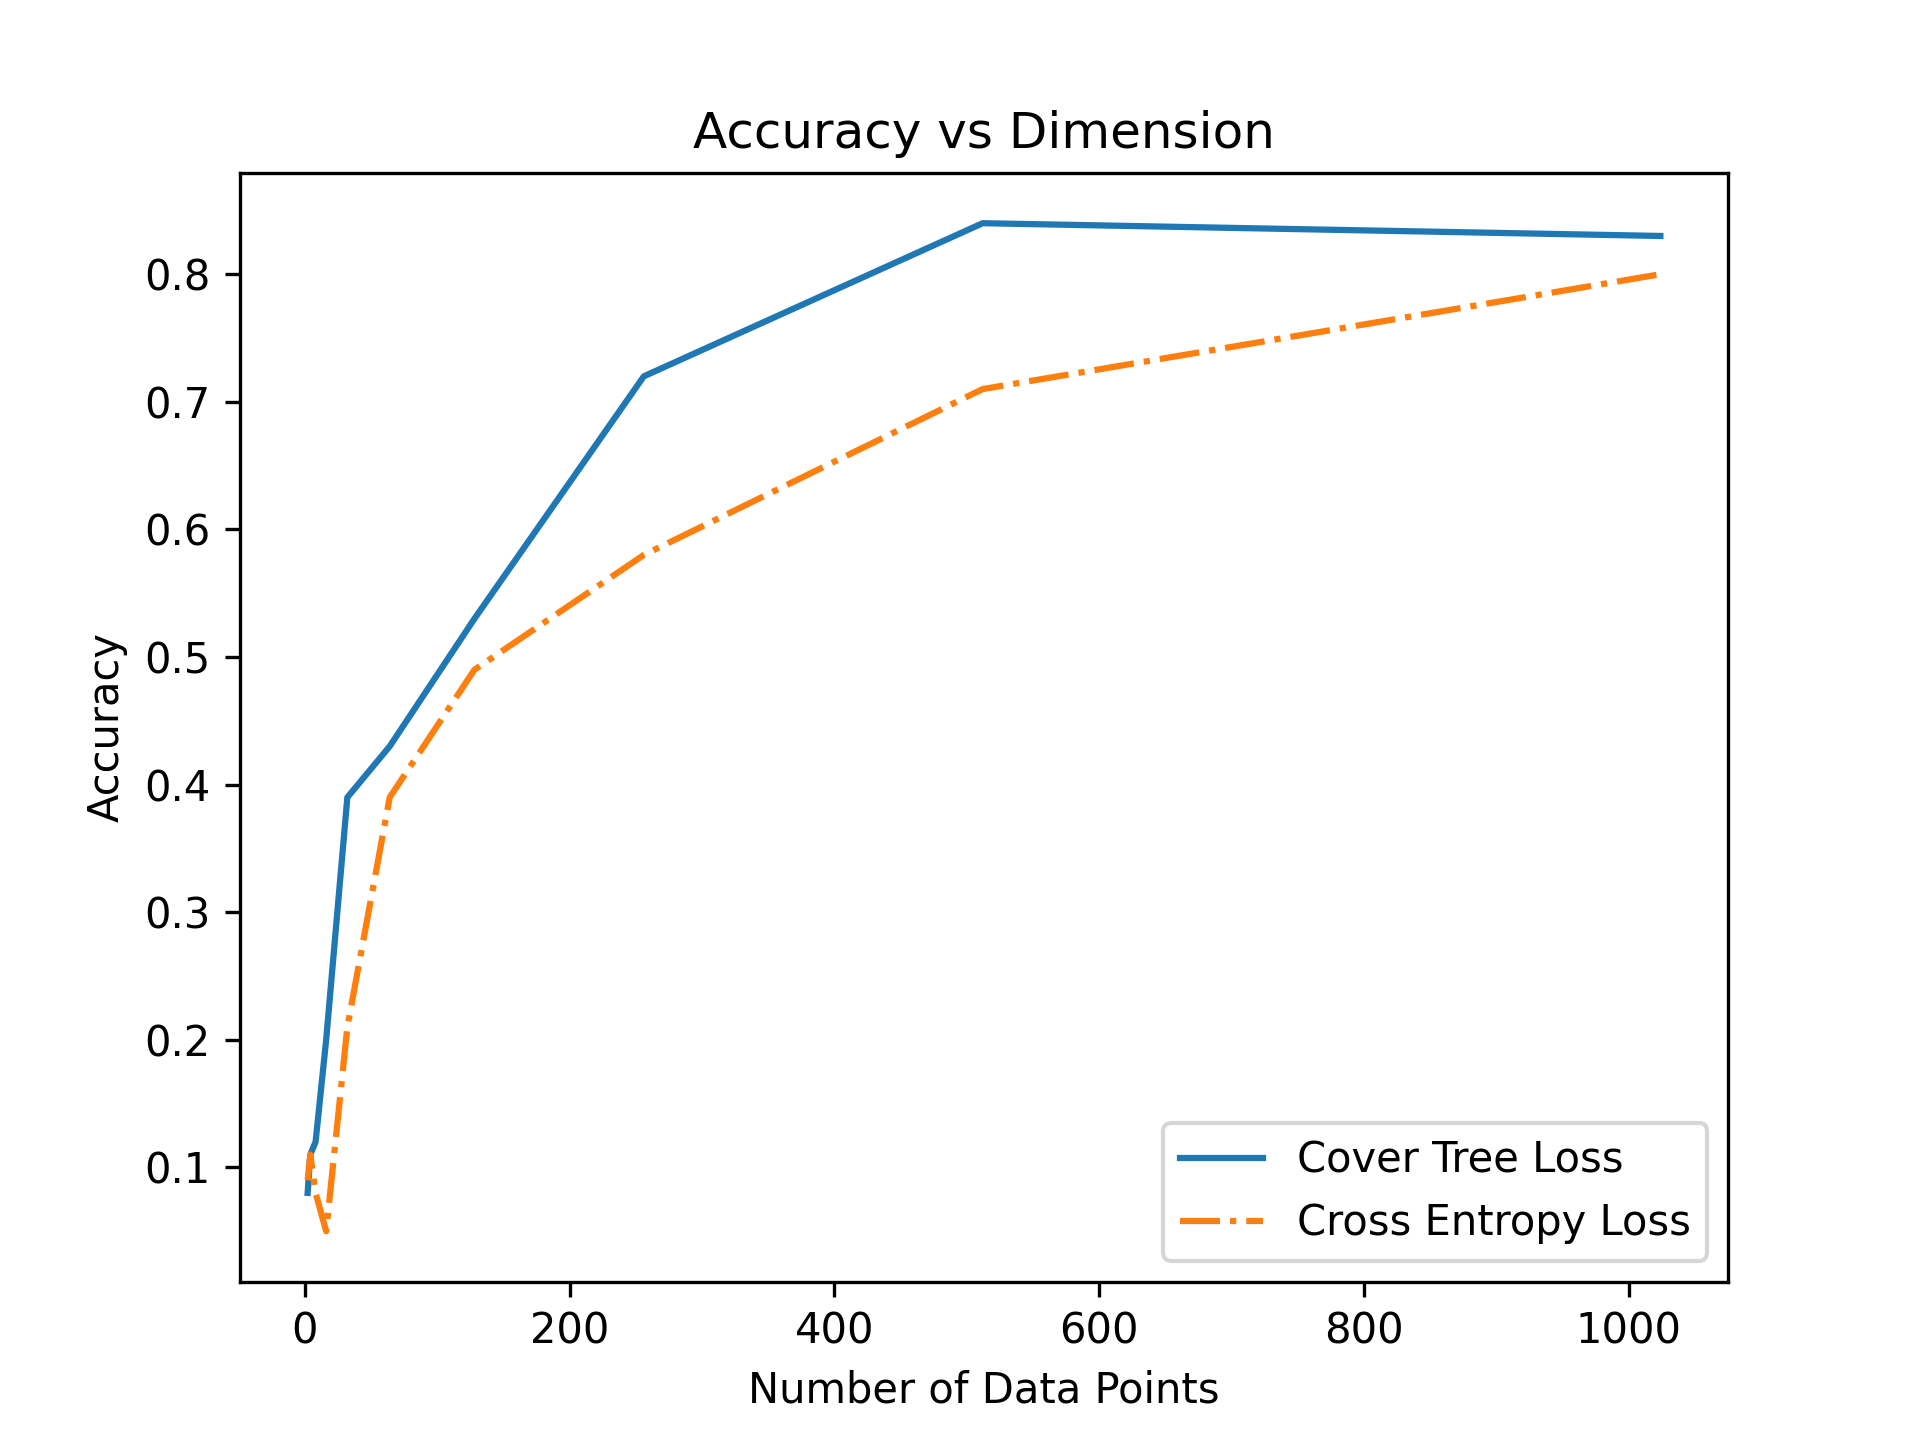
\includegraphics[width=0.48\columnwidth]{fig/images/accuracy_vs_d.png}
%
%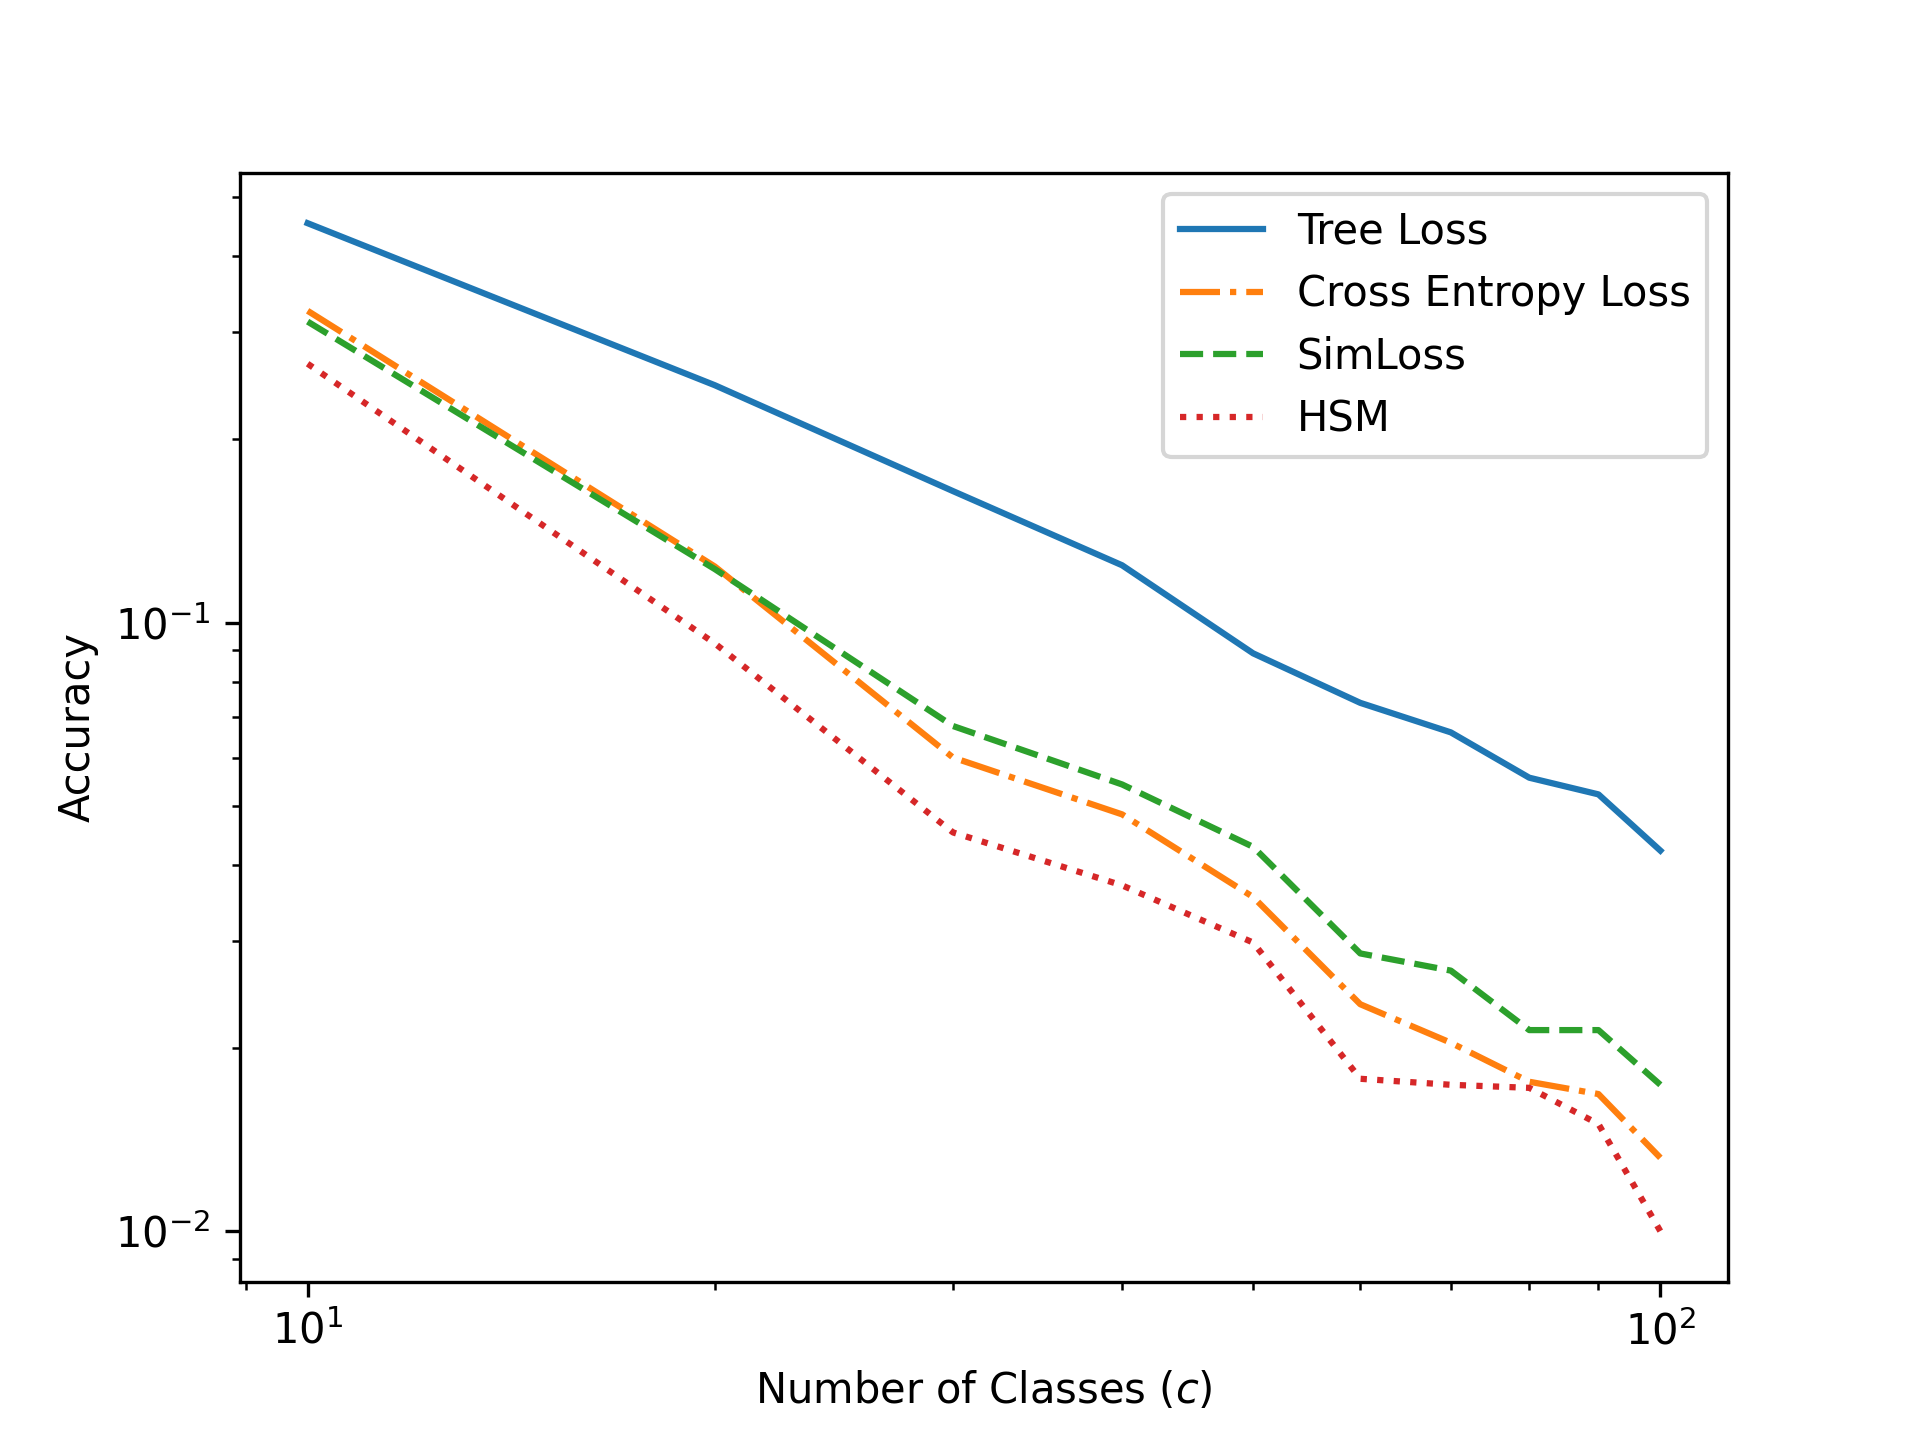
\includegraphics[width=0.48\columnwidth]{fig/images/accuracy_vs_class.png}
%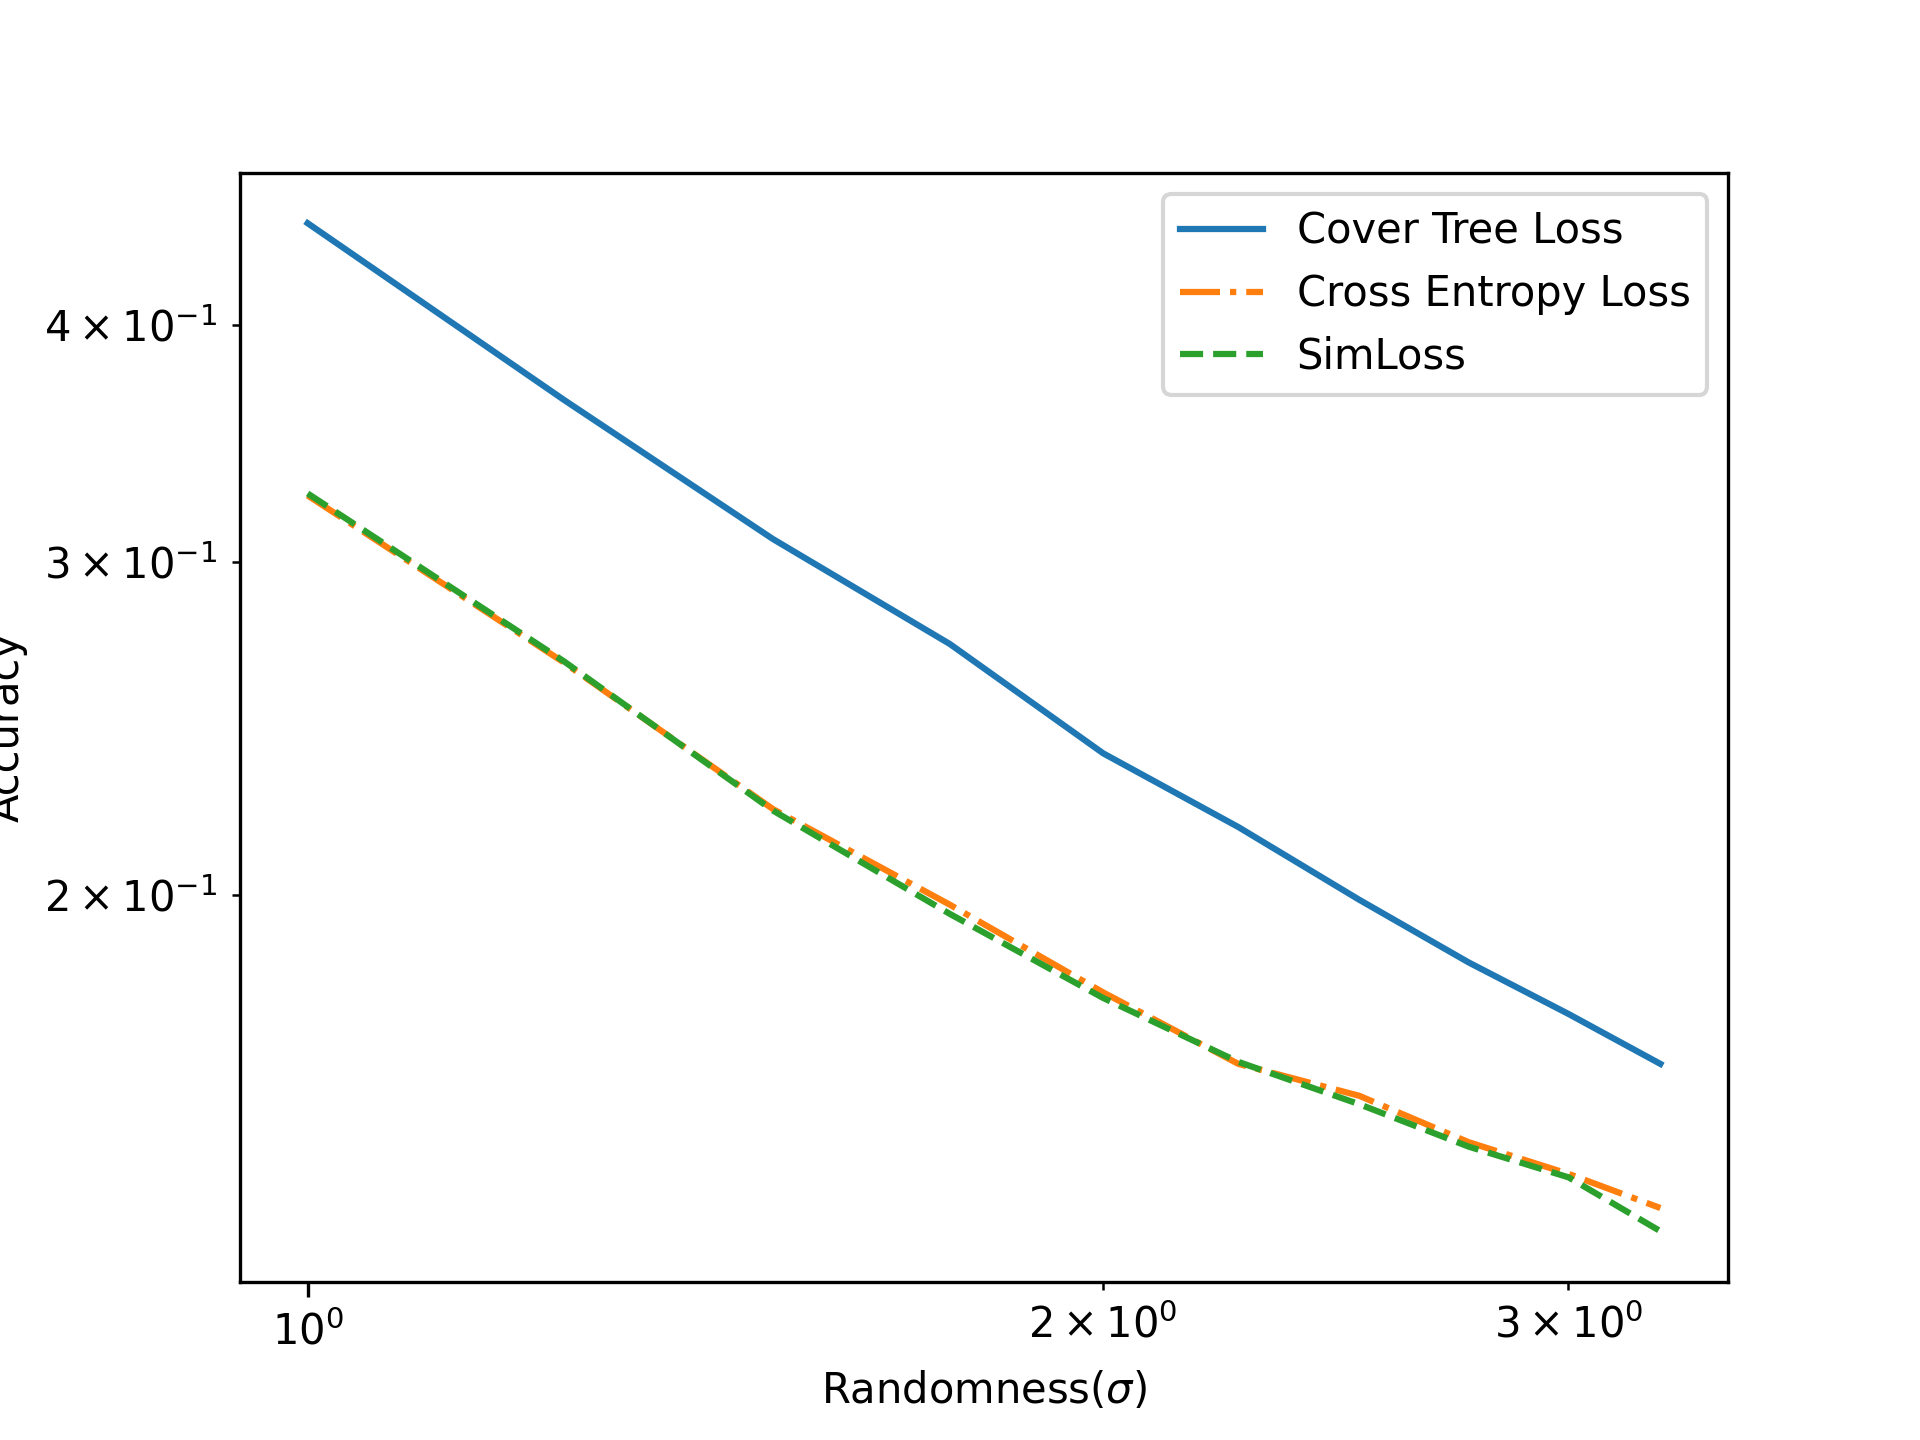
\includegraphics[width=0.48\columnwidth]{fig/images/accuracy_vs_sigma.png}

%%%%%%%%%%%%%%%%%%%%%%%%%%%%%%%%%%%%%%%%%%%%%%%%%%%%%%%%%%%%%%%%%%%%%%%%%%%%%%%%

\begin{frame}{Experiments: Synthetic: Ablation}
\begin{center}
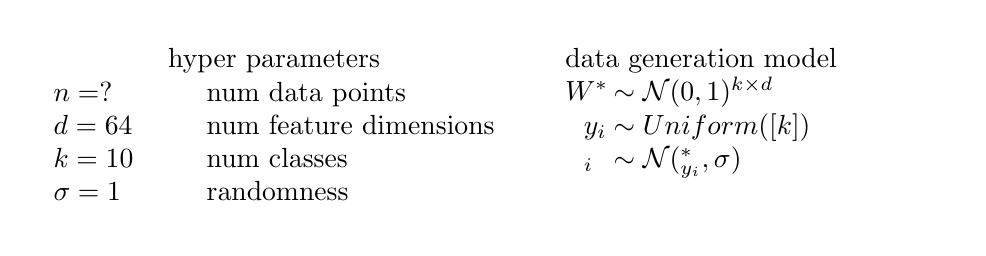
\begin{tikzpicture}
    \node[minimum height=1in]{\parbox{2in}{
        \begin{tabular}{p{0.6in}l}
            \multicolumn{2}{c}{hyper parameters} \\
            \midrule
            $n=?$ & num data points \\
            $d=64$ & num feature dimensions \\
            $k=10$ & num classes \\
            $\sigma=1$ & randomness \\
        \end{tabular}
    }};
    \node[minimum height=1in] at (6.5,0) {\parbox{2in}{
        \begin{tabular}{ll}
            \multicolumn{2}{c}{data generation model} \\
            \midrule
            $W^*$ & \!\!\!\!\!\!$\sim \mathcal N(0,1)^{k\times d}$ \\
            ~~$y_i$ & \!\!\!\!\!\!$\sim \text{Uniform}([k])$ \\
            ~~$\x_i$ & \!\!\!\!\!\!$\sim \mathcal N(\w^*_{y_i}, \sigma)$ \\
            \\
        \end{tabular}
    }};
\end{tikzpicture}
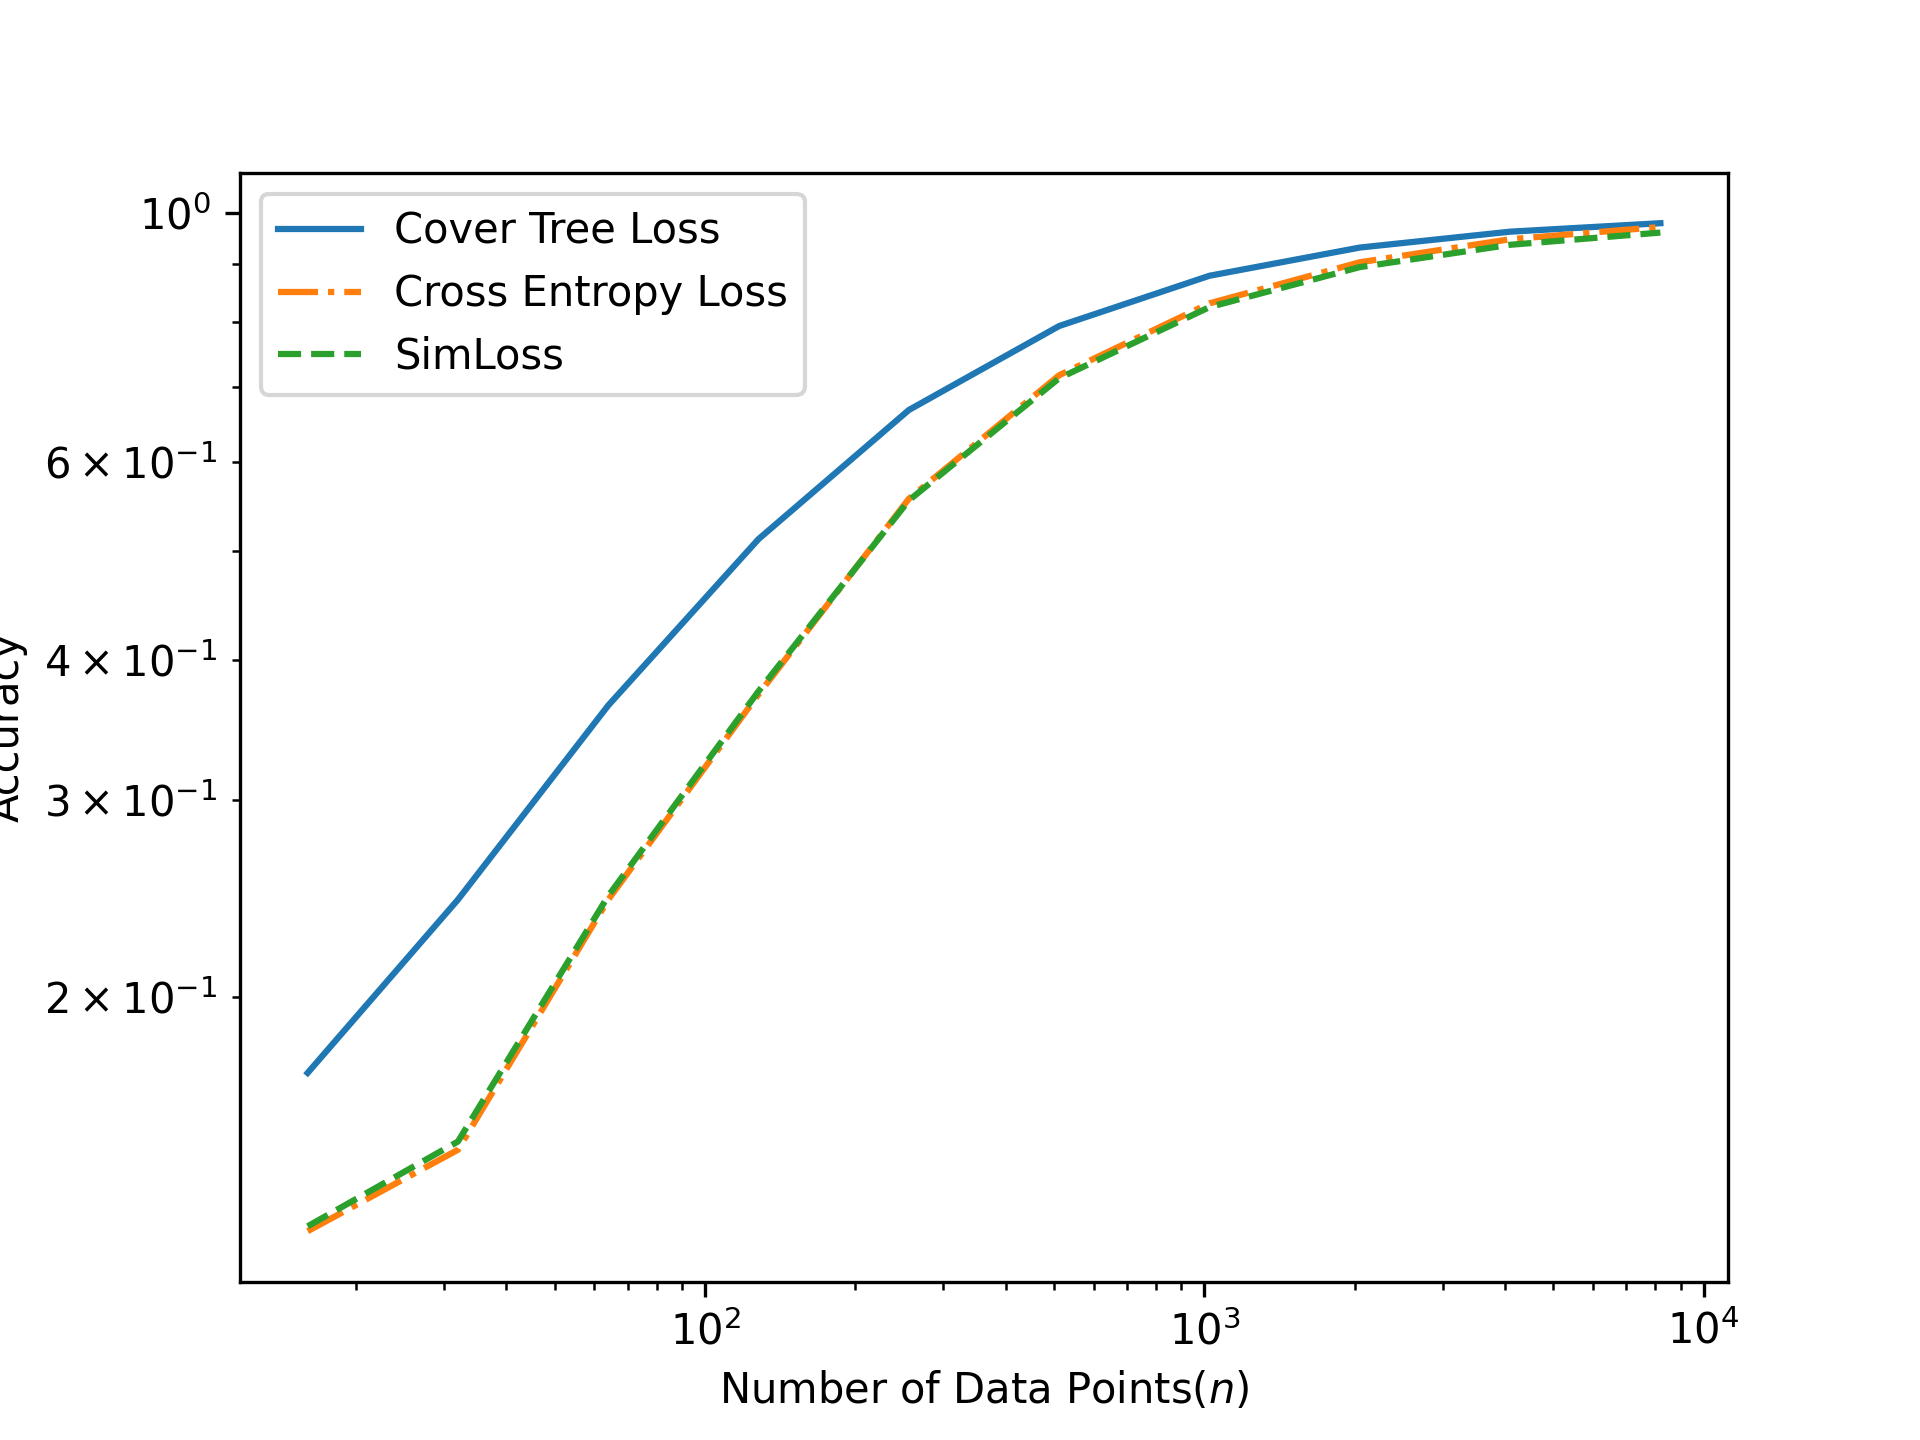
\includegraphics[width=0.8\columnwidth]{fig/images/accuracy_vs_n.png}
\end{center}
\end{frame}

%%%%%%%%%%%%%%%%%%%%

\begin{frame}{Experiments: Synthetic: Ablation}
\begin{center}
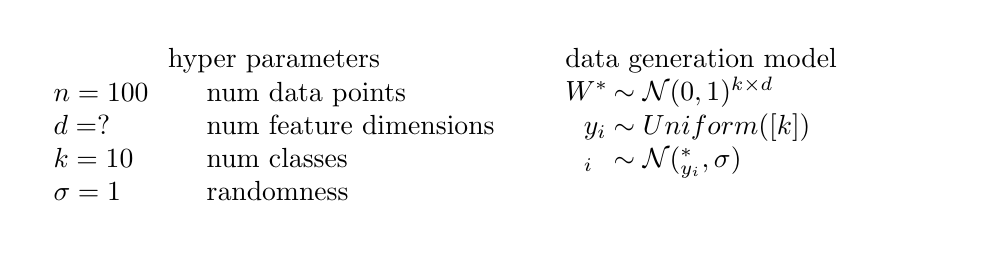
\begin{tikzpicture}
    \node[minimum height=1in]{\parbox{2in}{
        \begin{tabular}{p{0.6in}l}
            \multicolumn{2}{c}{hyper parameters} \\
            \midrule
            $n=100$ & num data points \\
            $d=?$ & num feature dimensions \\
            $k=10$ & num classes \\
            $\sigma=1$ & randomness \\
        \end{tabular}
    }};
    \node[minimum height=1in] at (6.5,0) {\parbox{2in}{
        \begin{tabular}{ll}
            \multicolumn{2}{c}{data generation model} \\
            \midrule
            $W^*$ & \!\!\!\!\!\!$\sim \mathcal N(0,1)^{k\times d}$ \\
            ~~$y_i$ & \!\!\!\!\!\!$\sim \text{Uniform}([k])$ \\
            ~~$\x_i$ & \!\!\!\!\!\!$\sim \mathcal N(\w^*_{y_i}, \sigma)$ \\
            \\
        \end{tabular}
    }};
\end{tikzpicture}
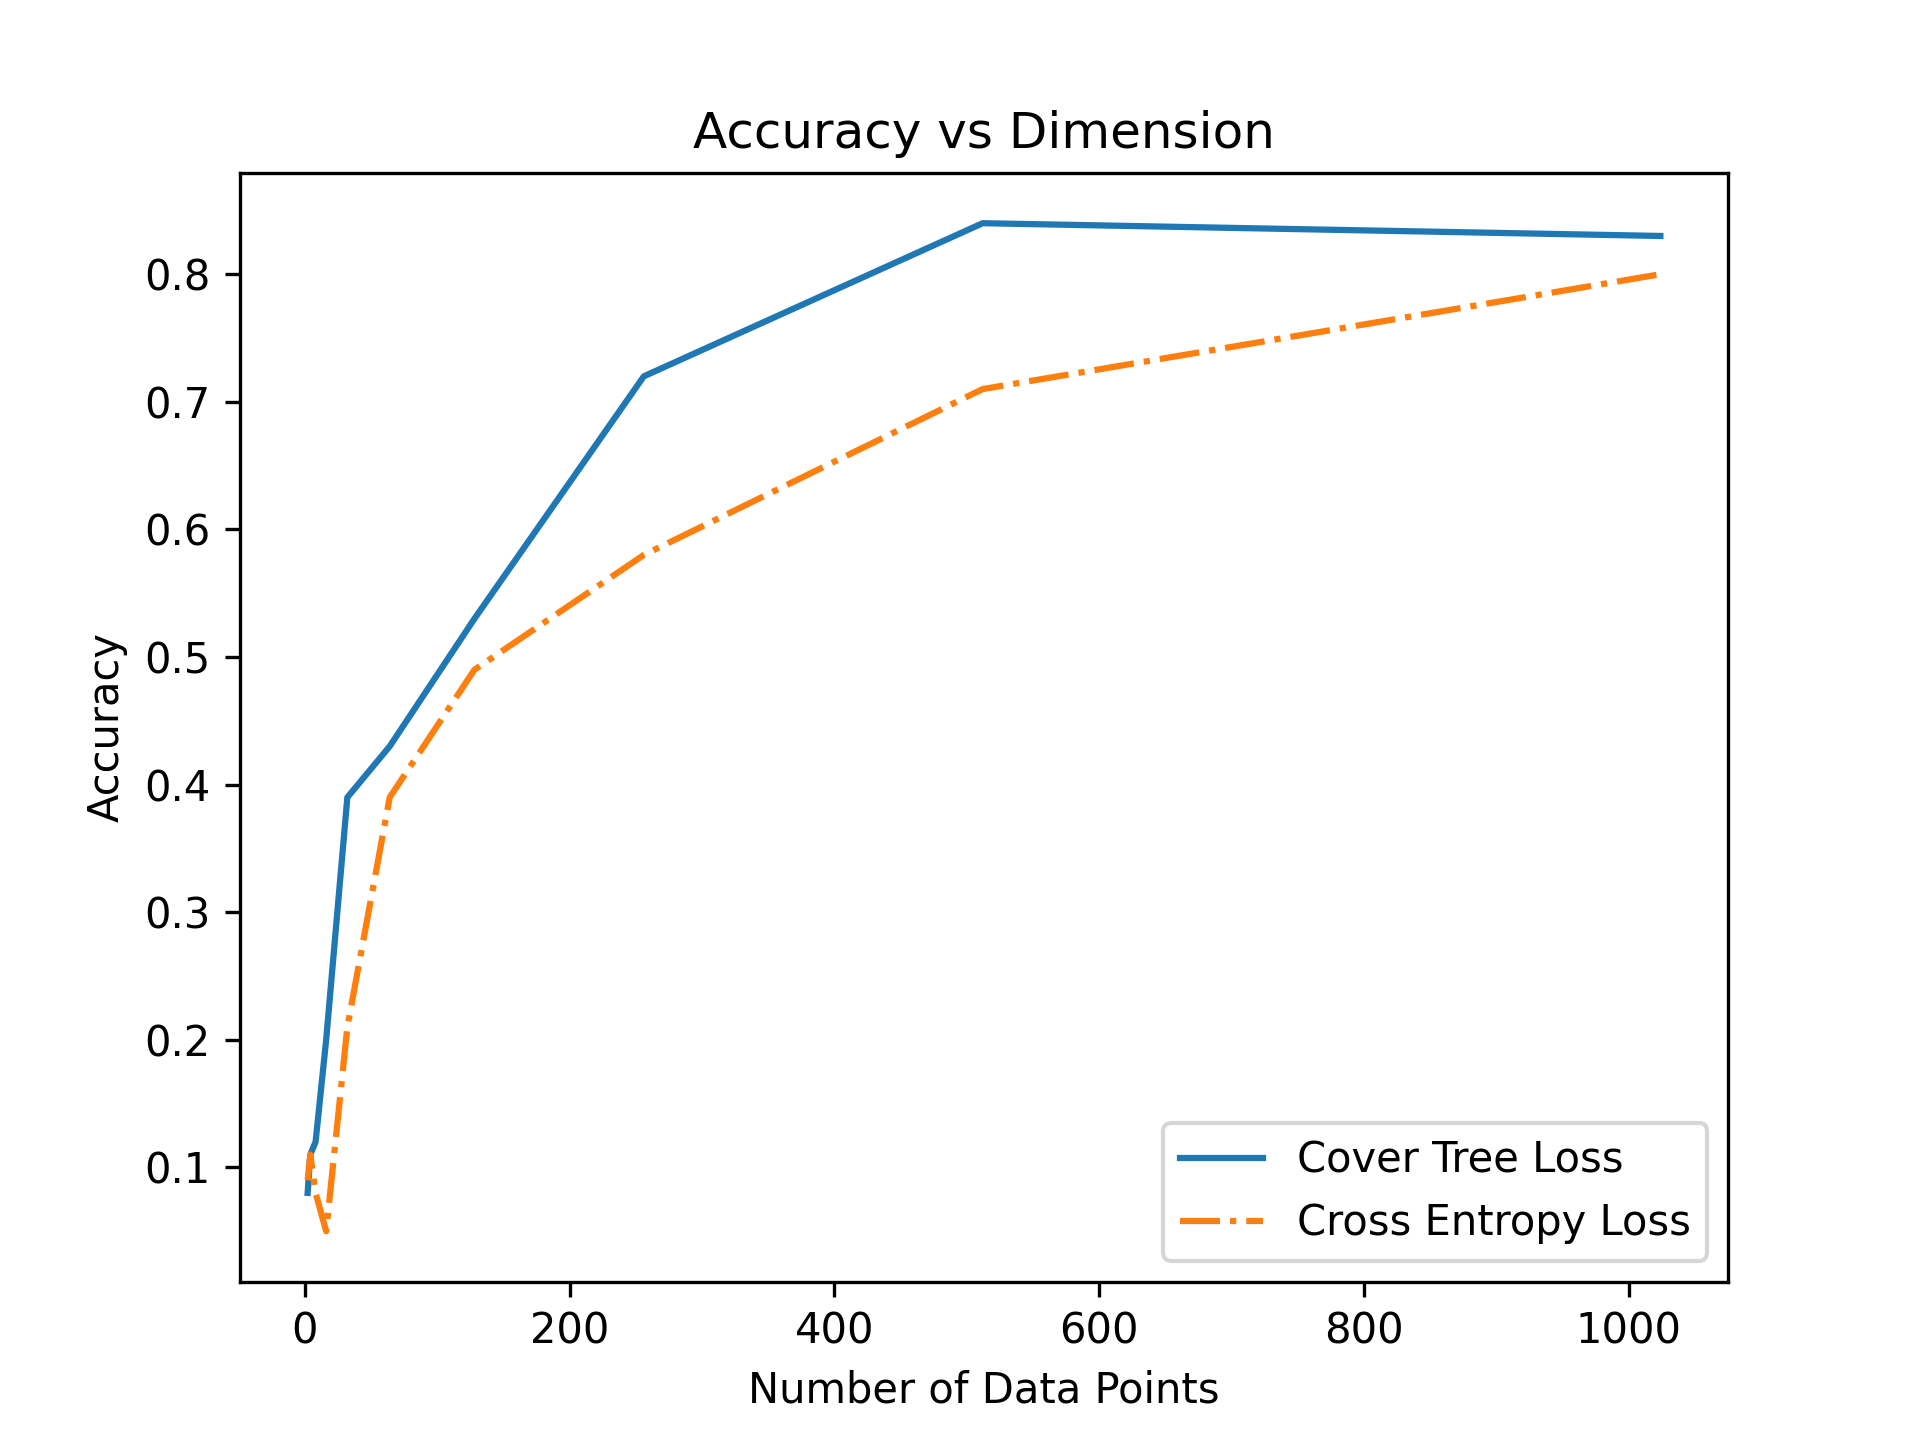
\includegraphics[width=0.8\columnwidth]{fig/images/accuracy_vs_d.png}
\end{center}
\end{frame}

%%%%%%%%%%%%%%%%%%%%

\begin{frame}{Experiments: Synthetic: Ablation}
\begin{center}
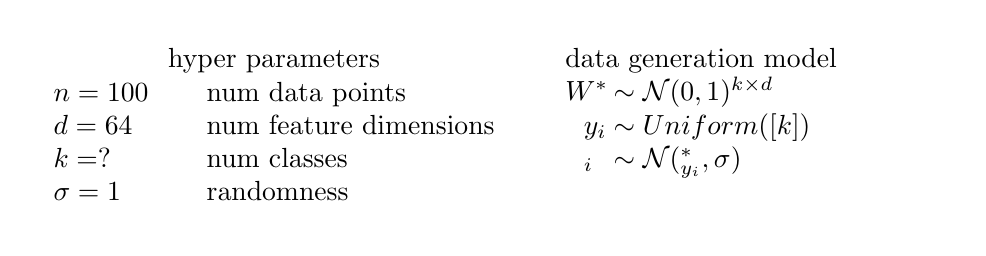
\begin{tikzpicture}
    \node[minimum height=1in]{\parbox{2in}{
        \begin{tabular}{p{0.6in}l}
            \multicolumn{2}{c}{hyper parameters} \\
            \midrule
            $n=100$ & num data points \\
            $d=64$ & num feature dimensions \\
            $k=?$ & num classes \\
            $\sigma=1$ & randomness \\
        \end{tabular}
    }};
    \node[minimum height=1in] at (6.5,0) {\parbox{2in}{
        \begin{tabular}{ll}
            \multicolumn{2}{c}{data generation model} \\
            \midrule
            $W^*$ & \!\!\!\!\!\!$\sim \mathcal N(0,1)^{k\times d}$ \\
            ~~$y_i$ & \!\!\!\!\!\!$\sim \text{Uniform}([k])$ \\
            ~~$\x_i$ & \!\!\!\!\!\!$\sim \mathcal N(\w^*_{y_i}, \sigma)$ \\
            \\
        \end{tabular}
    }};
\end{tikzpicture}
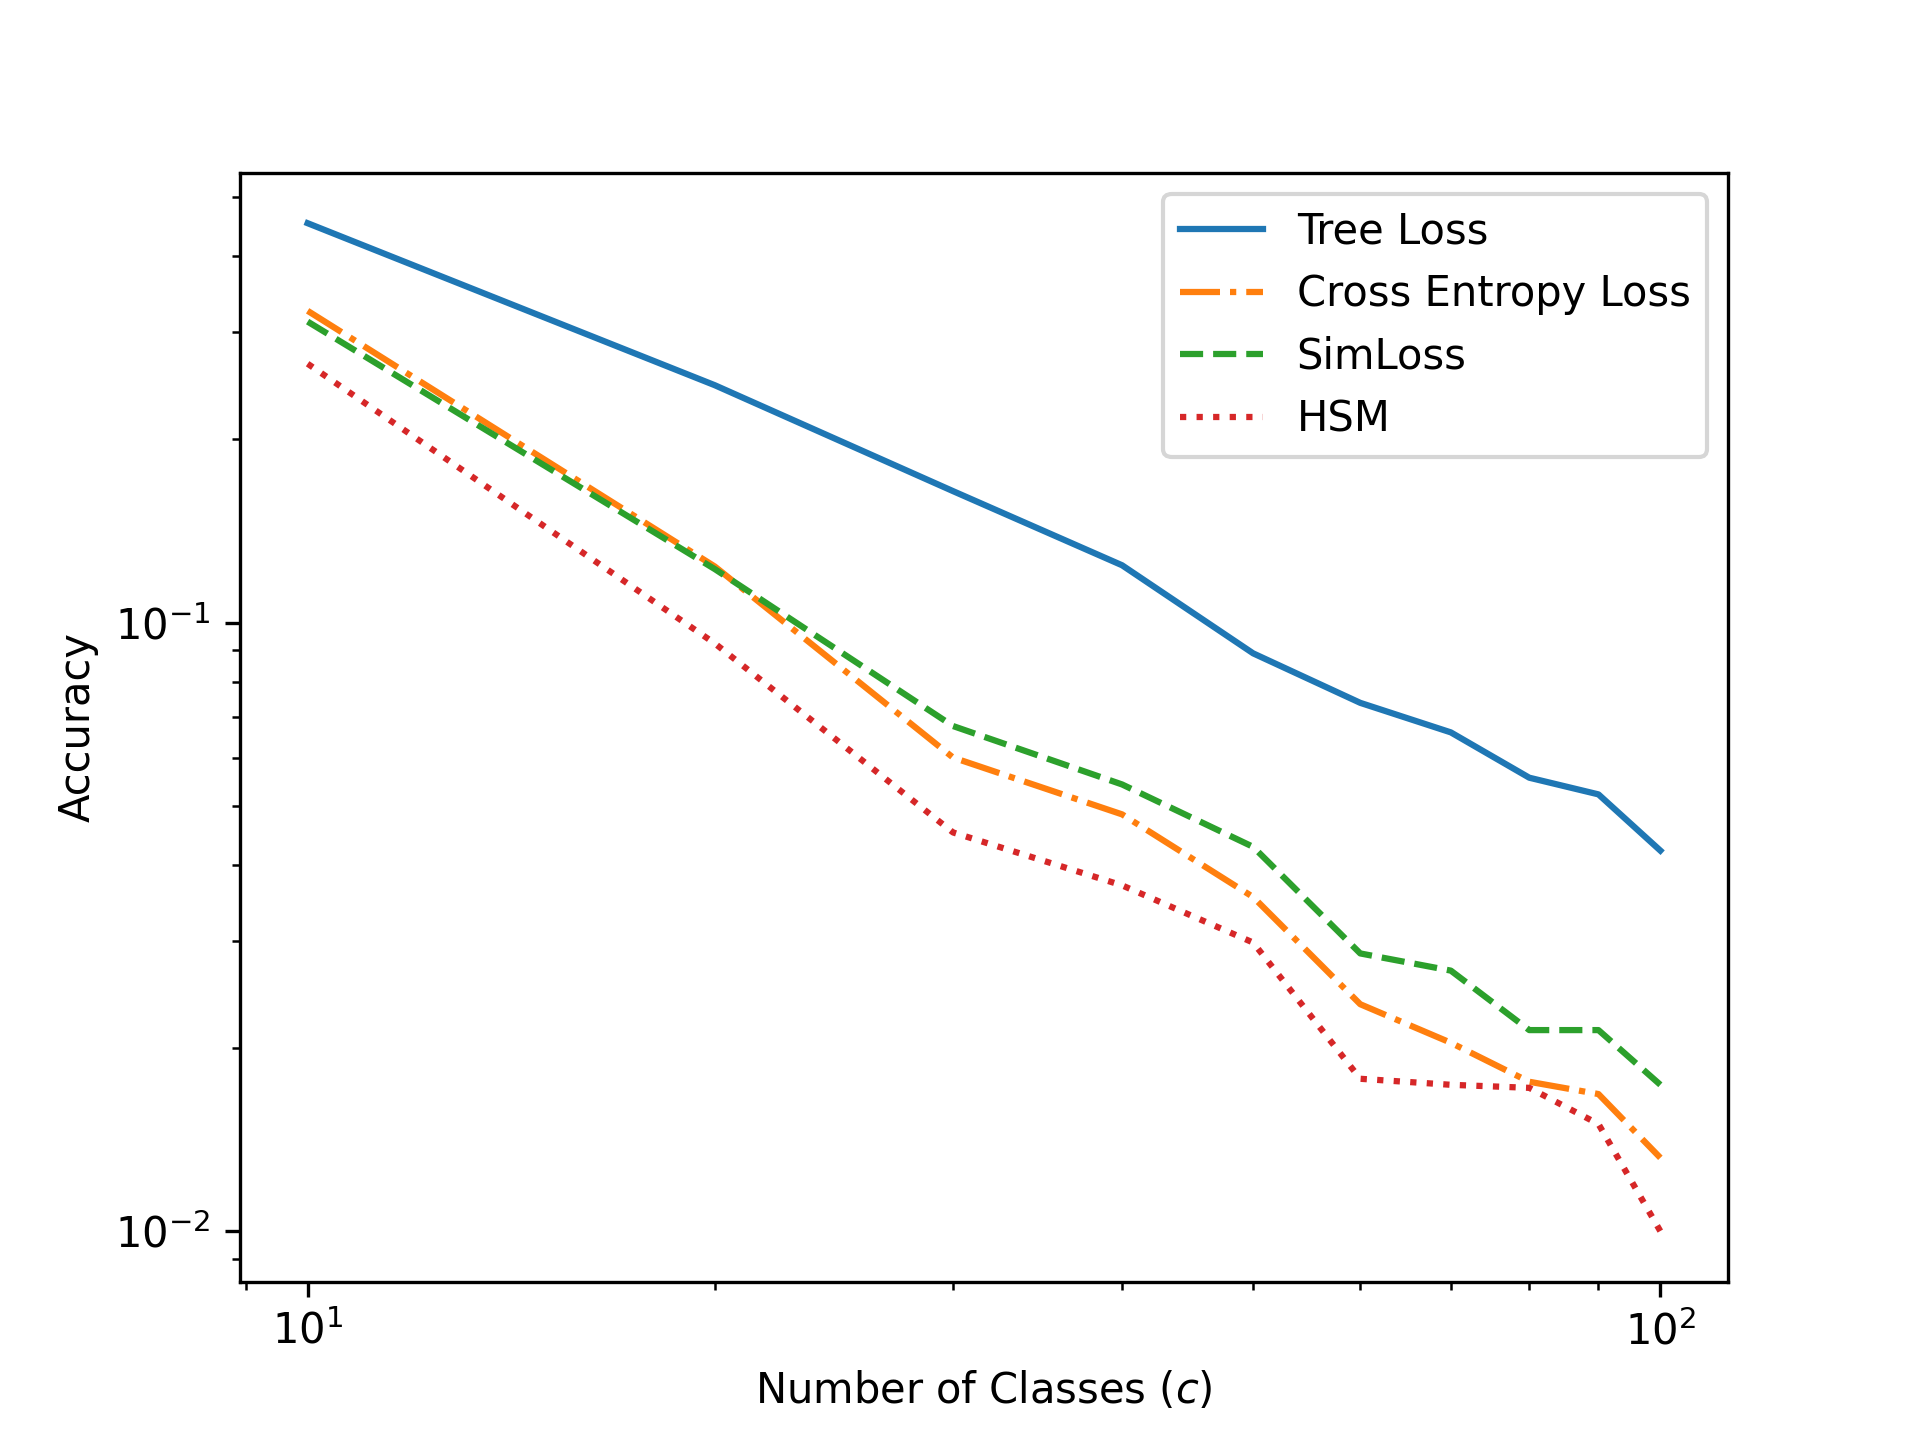
\includegraphics[width=0.8\columnwidth]{fig/images/accuracy_vs_class.png}
\end{center}
\end{frame}

%%%%%%%%%%%%%%%%%%%%

\begin{frame}{Experiments: Synthetic: Ablation}
\begin{center}
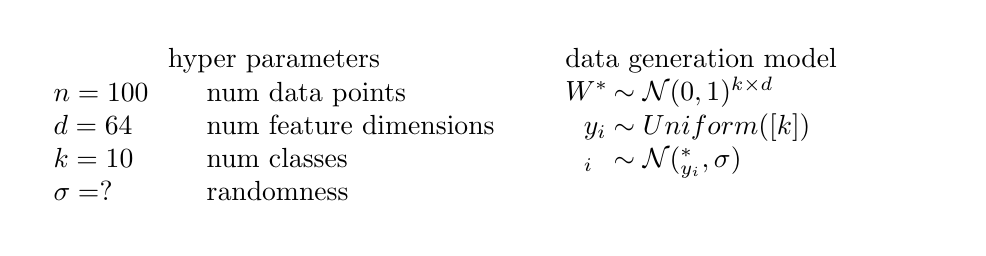
\begin{tikzpicture}
    \node[minimum height=1in]{\parbox{2in}{
        \begin{tabular}{p{0.6in}l}
            \multicolumn{2}{c}{hyper parameters} \\
            \midrule
            $n=100$ & num data points \\
            $d=64$ & num feature dimensions \\
            $k=10$ & num classes \\
            $\sigma=?$ & randomness \\
        \end{tabular}
    }};
    \node[minimum height=1in] at (6.5,0) {\parbox{2in}{
        \begin{tabular}{ll}
            \multicolumn{2}{c}{data generation model} \\
            \midrule
            $W^*$ & \!\!\!\!\!\!$\sim \mathcal N(0,1)^{k\times d}$ \\
            ~~$y_i$ & \!\!\!\!\!\!$\sim \text{Uniform}([k])$ \\
            ~~$\x_i$ & \!\!\!\!\!\!$\sim \mathcal N(\w^*_{y_i}, \sigma)$ \\
            \\
        \end{tabular}
    }};
\end{tikzpicture}
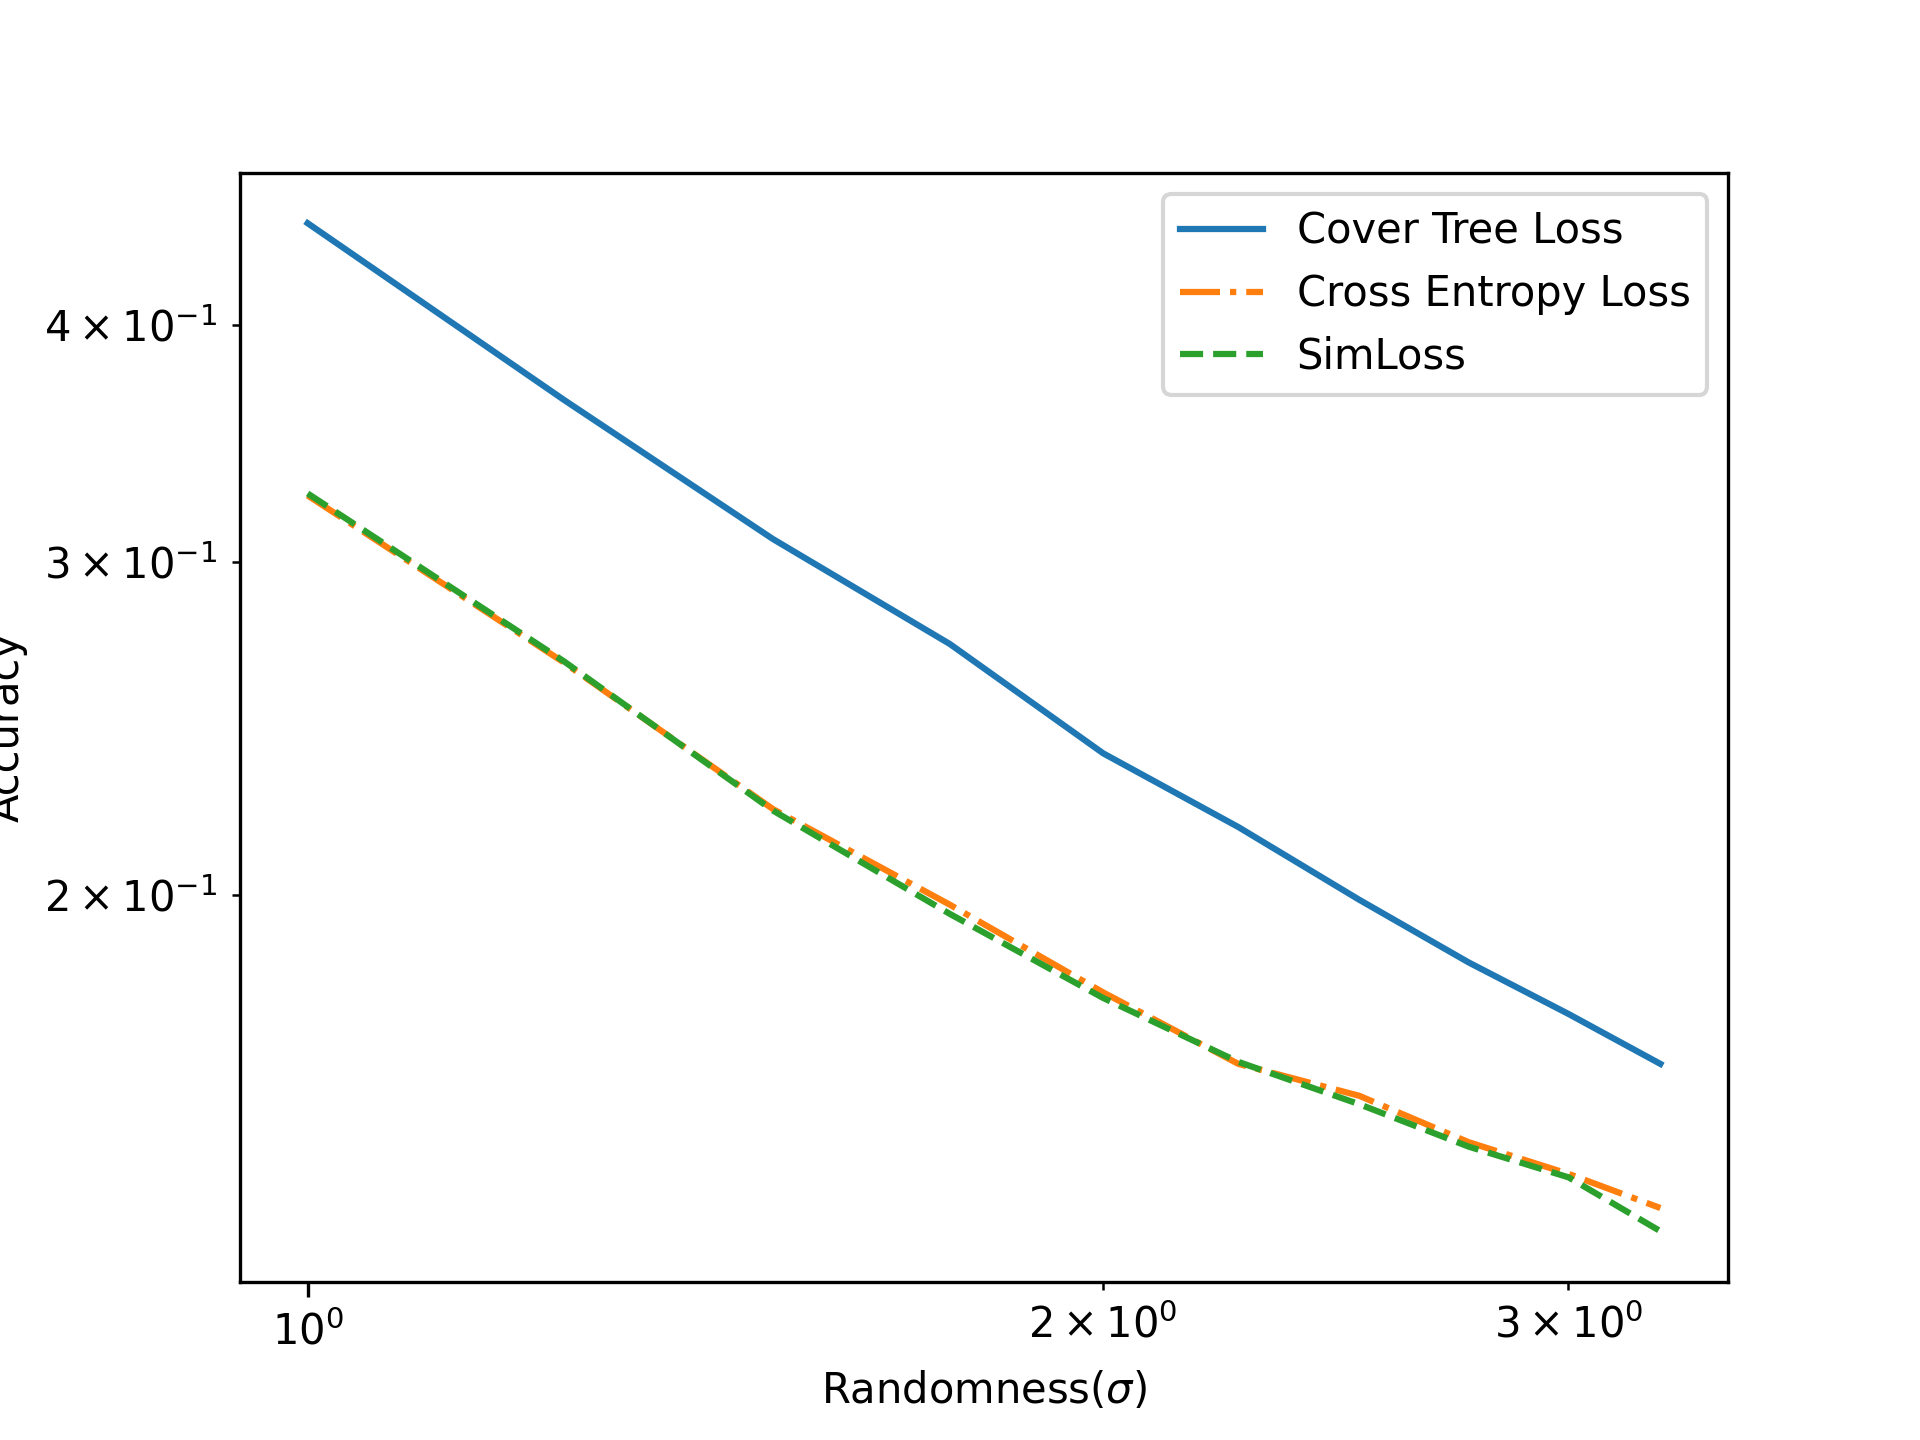
\includegraphics[width=0.8\columnwidth]{fig/images/accuracy_vs_sigma.png}
\end{center}
\end{frame}

%%%%%%%%%%%%%%%%%%%%

\begin{frame}{Experiments: Synthetic: Lemma Verification}
\begin{center}
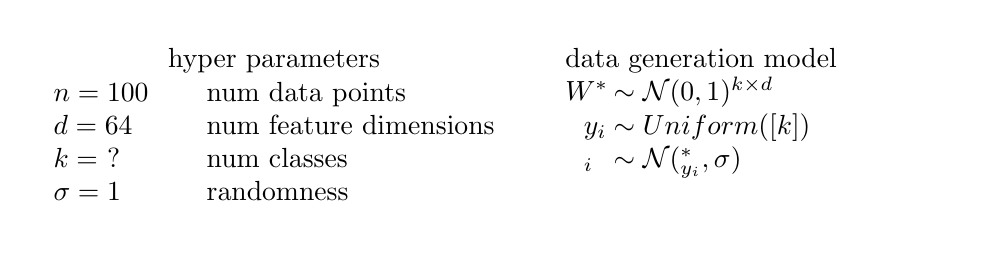
\begin{tikzpicture}
    \node[minimum height=1in]{\parbox{2in}{
        \begin{tabular}{p{0.6in}l}
            \multicolumn{2}{c}{hyper parameters} \\
            \midrule
            $n=100$ & num data points \\
            $d=64$ & num feature dimensions \\
            $k=~?$ & num classes \\
            $\sigma=1$ & randomness \\
        \end{tabular}
    }};
    \node[minimum height=1in] at (6.5,0) {\parbox{2in}{
        \begin{tabular}{ll}
            \multicolumn{2}{c}{data generation model} \\
            \midrule
            $W^*$ & \!\!\!\!\!\!$\sim \mathcal N(0,1)^{k\times d}$ \\
            ~~$y_i$ & \!\!\!\!\!\!$\sim \text{Uniform}([k])$ \\
            ~~$\x_i$ & \!\!\!\!\!\!$\sim \mathcal N(\w^*_{y_i}, \sigma)$ \\
            \\
        \end{tabular}
    }};
\end{tikzpicture}
%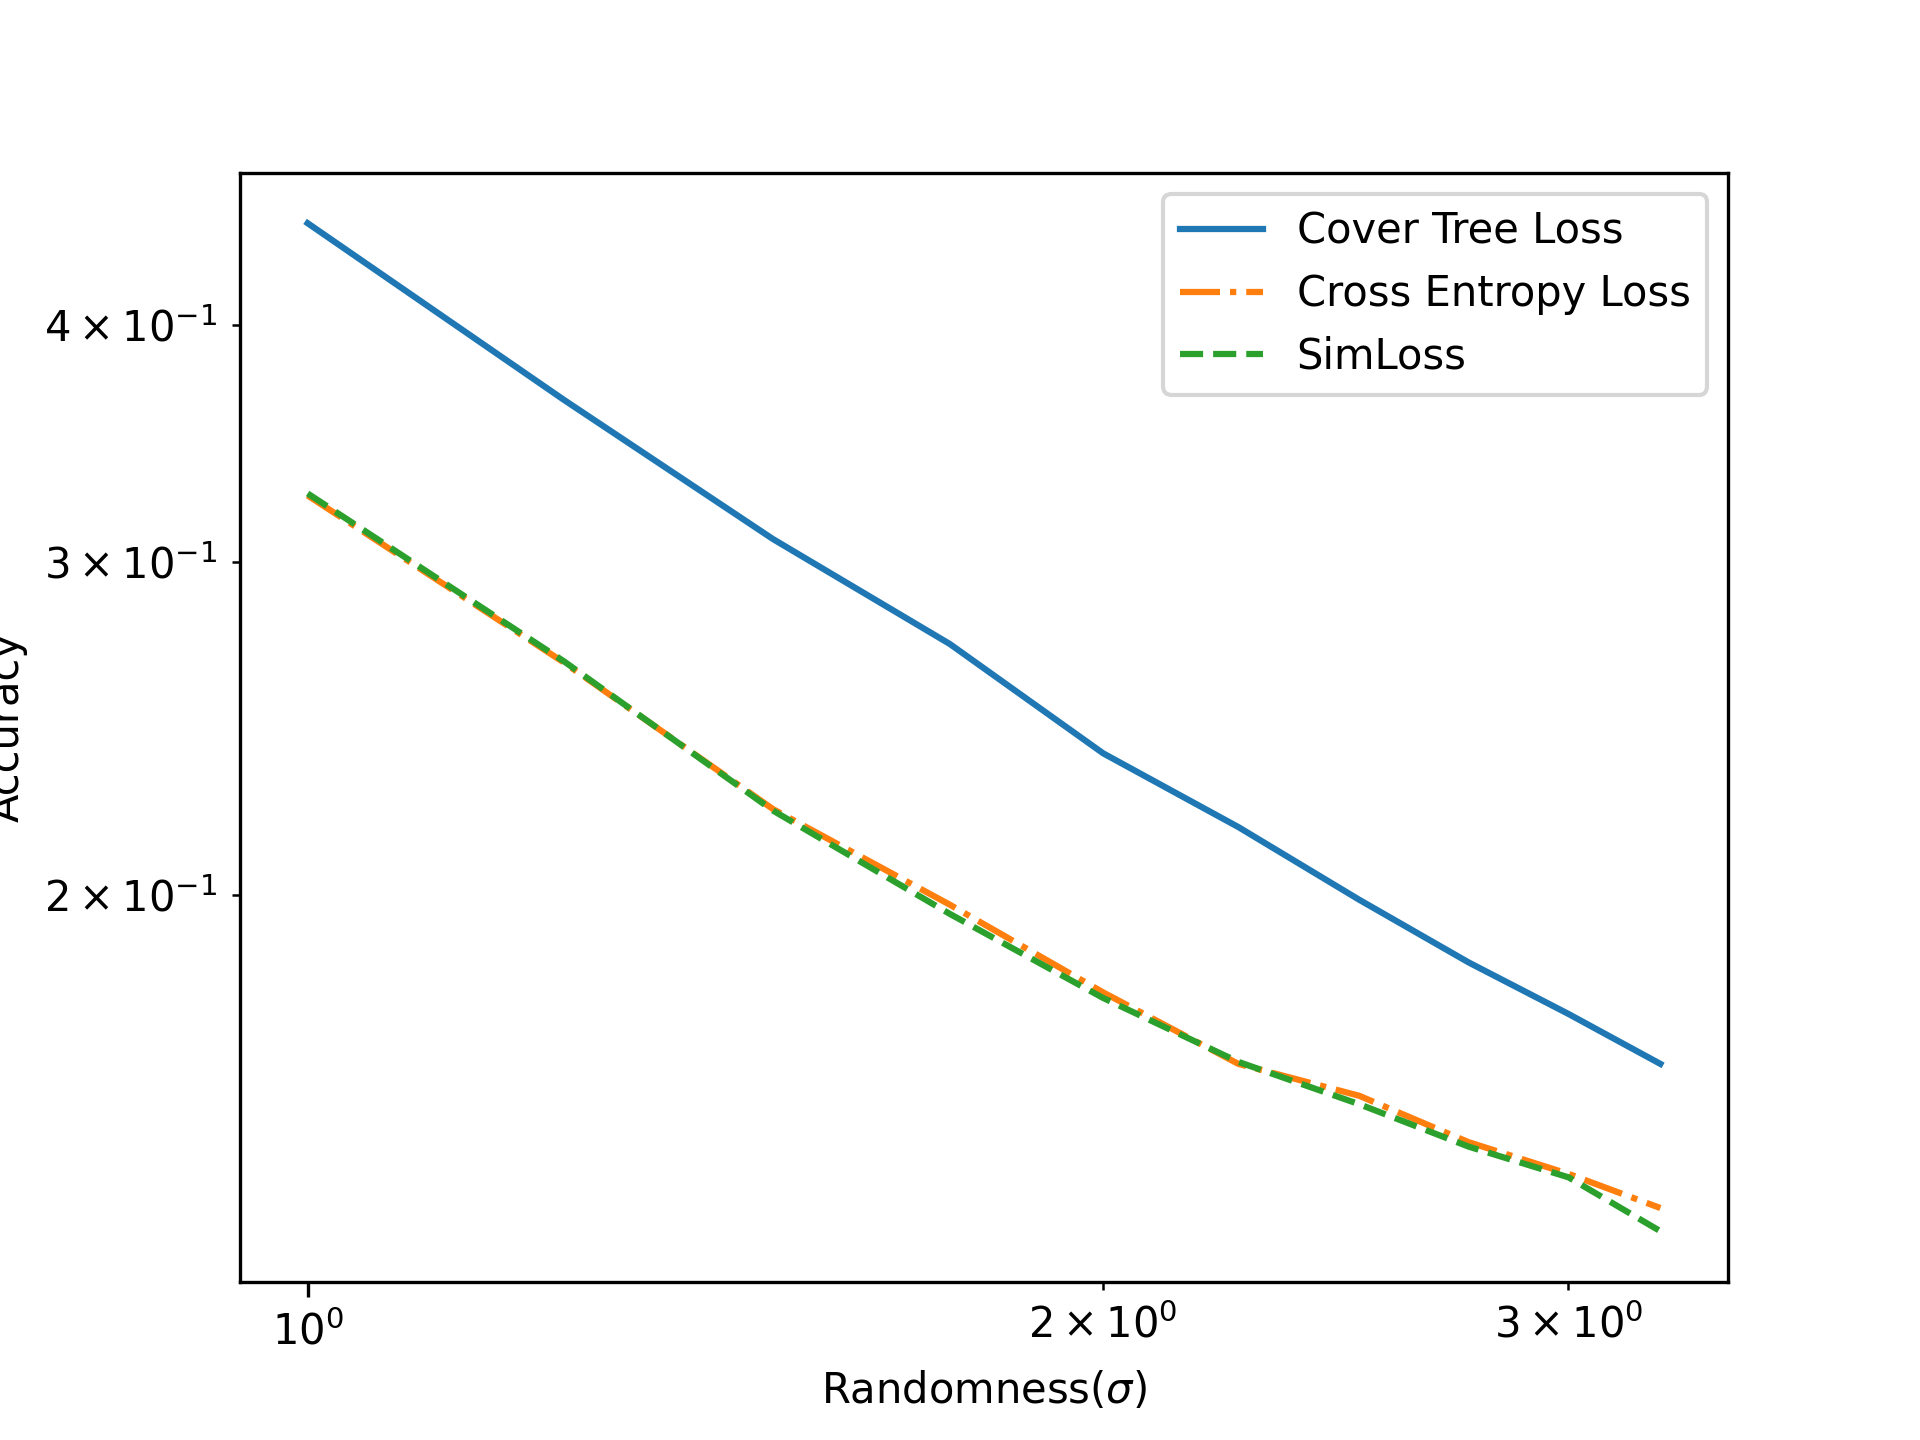
\includegraphics[width=0.8\columnwidth]{fig/images/accuracy_vs_sigma.png}
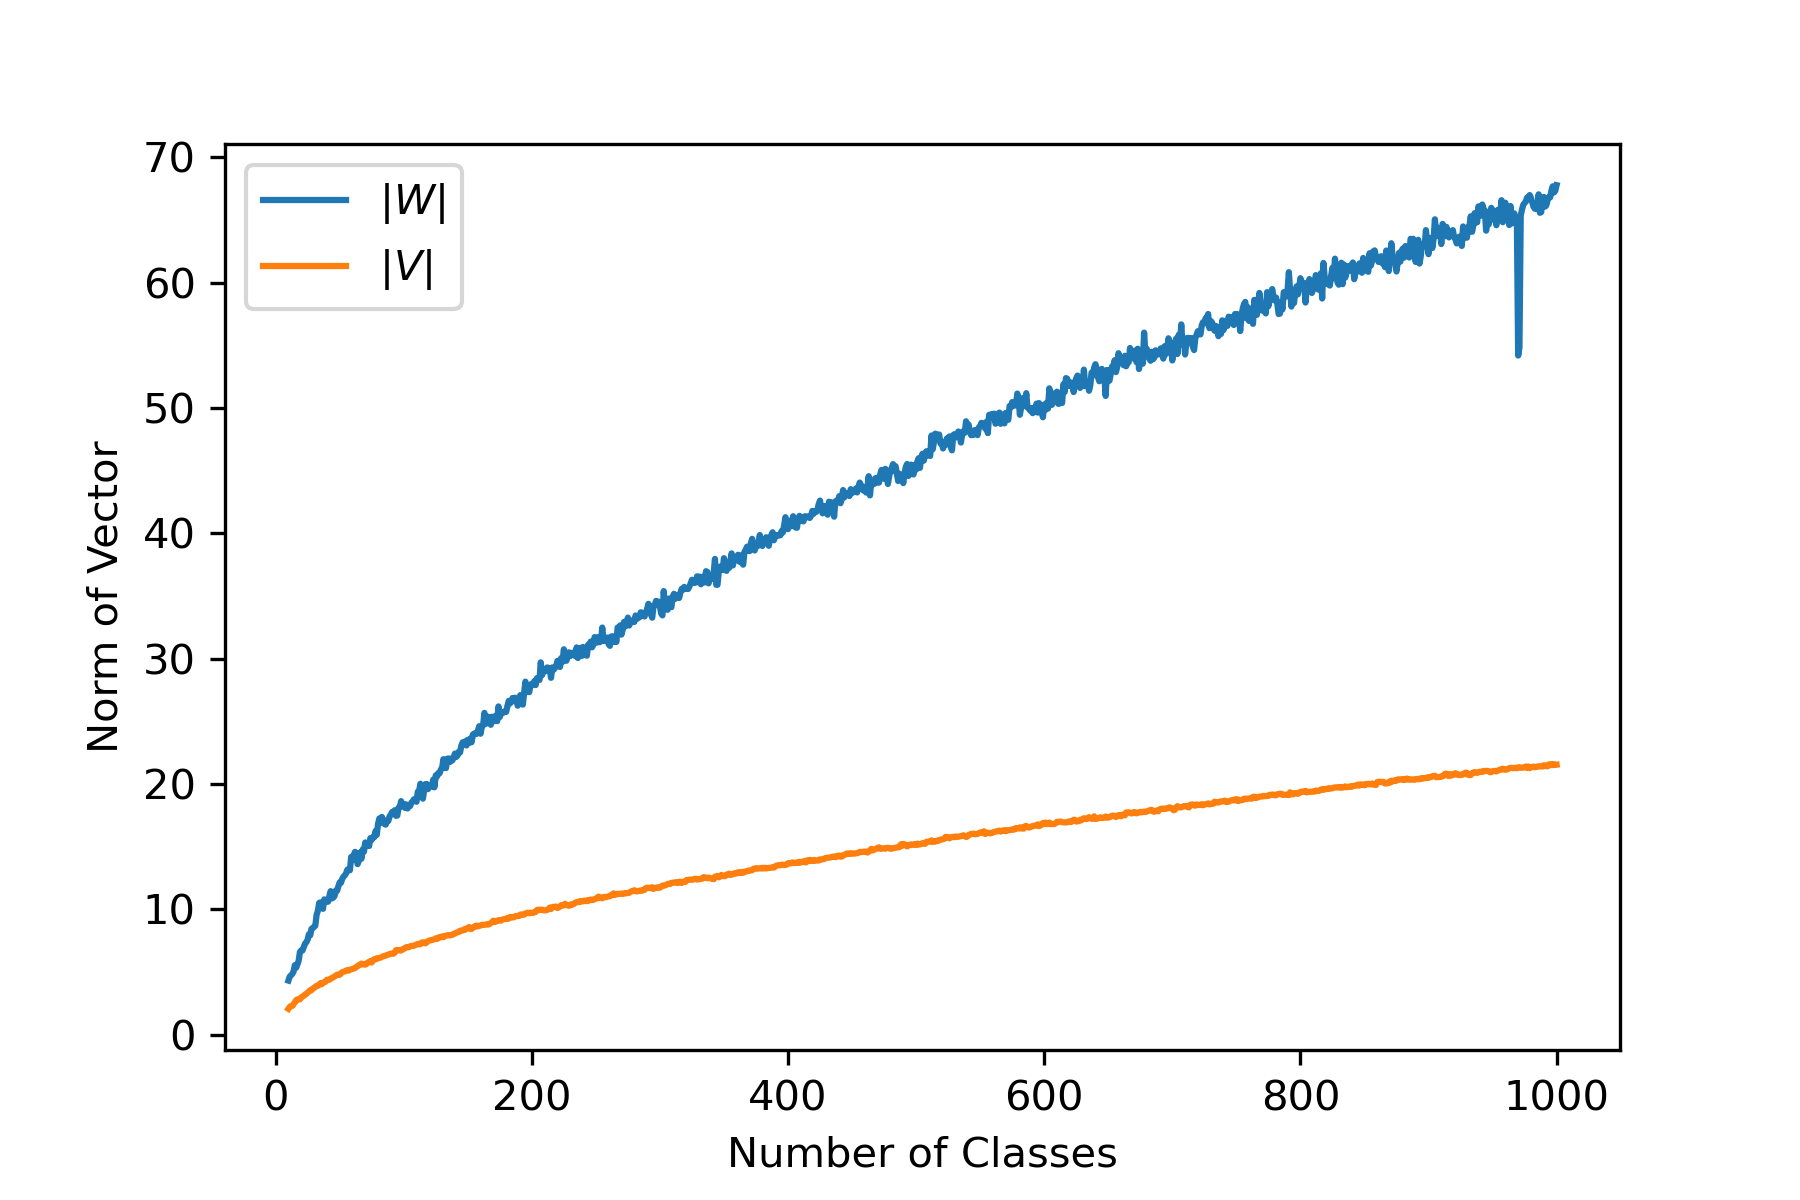
\includegraphics[width=0.8\columnwidth]{fig/images/class_v_norm.png}
\end{center}
\end{frame}


%%%%%%%%%%%%%%%%%%%%%%%%%%%%%%%%%%%%%%%%%%%%%%%%%%%%%%%%%%%%%%%%%%%%%%%%%%%%%%%%

%\begin{frame}{Experiments: Synthetic: Cover Tree}
%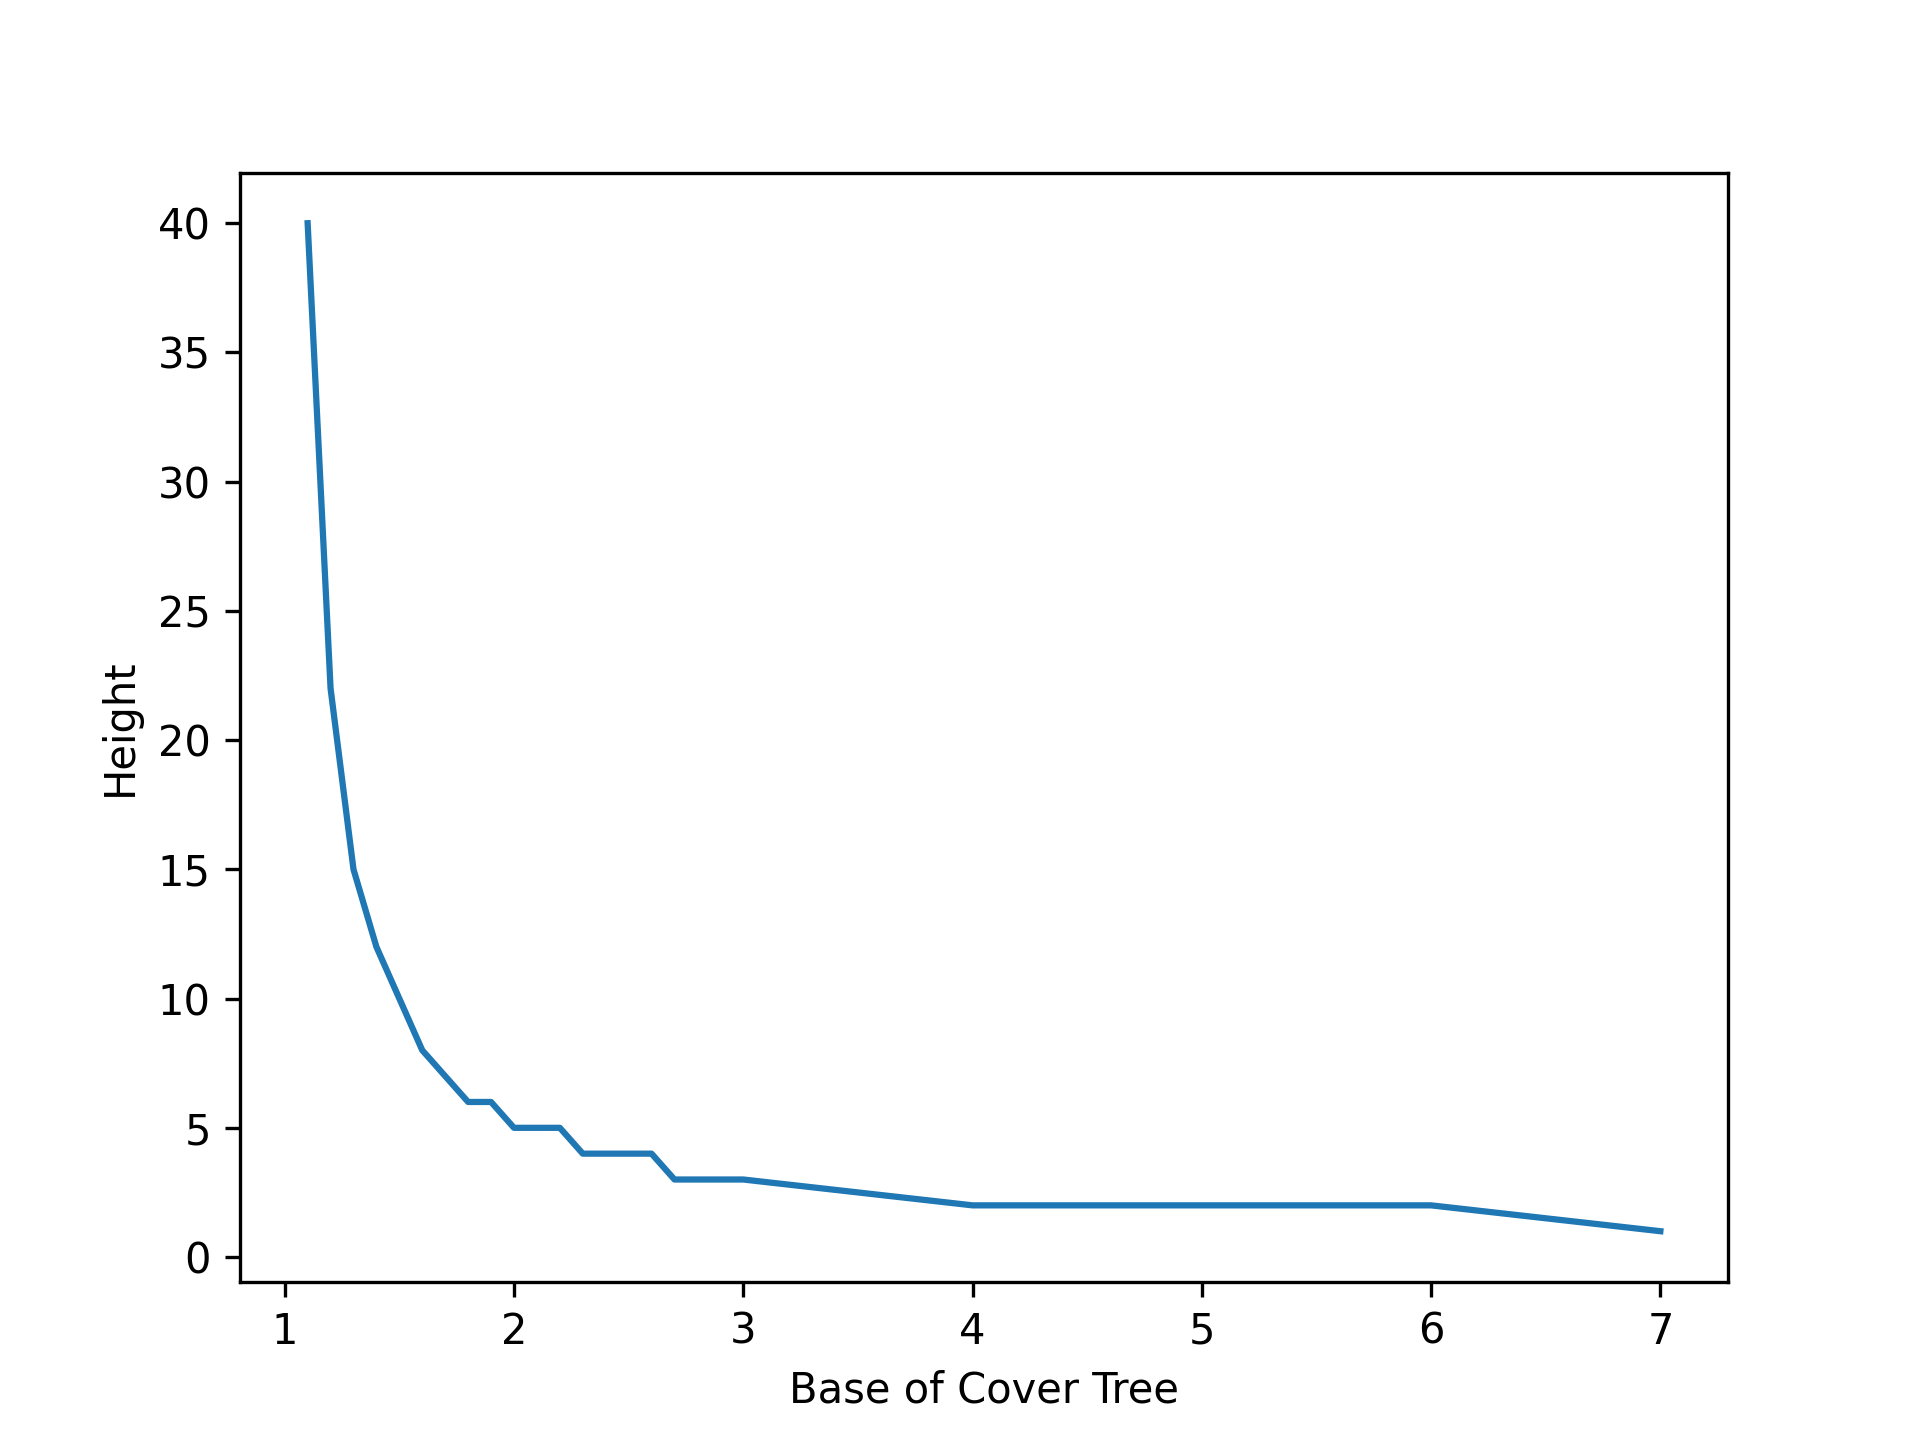
\includegraphics[width=\columnwidth]{fig/new_img/height_vs_base.png}
%\end{frame}

%%%%%%%%%%%%%%%%%%%%%%%%%%%%%%%%%%%%%%%%%%%%%%%%%%%%%%%%%%%%%%%%%%%%%%%%%%%%%%%%

%\begin{frame}{Experiments: Synthetic: Hyperparameters}
%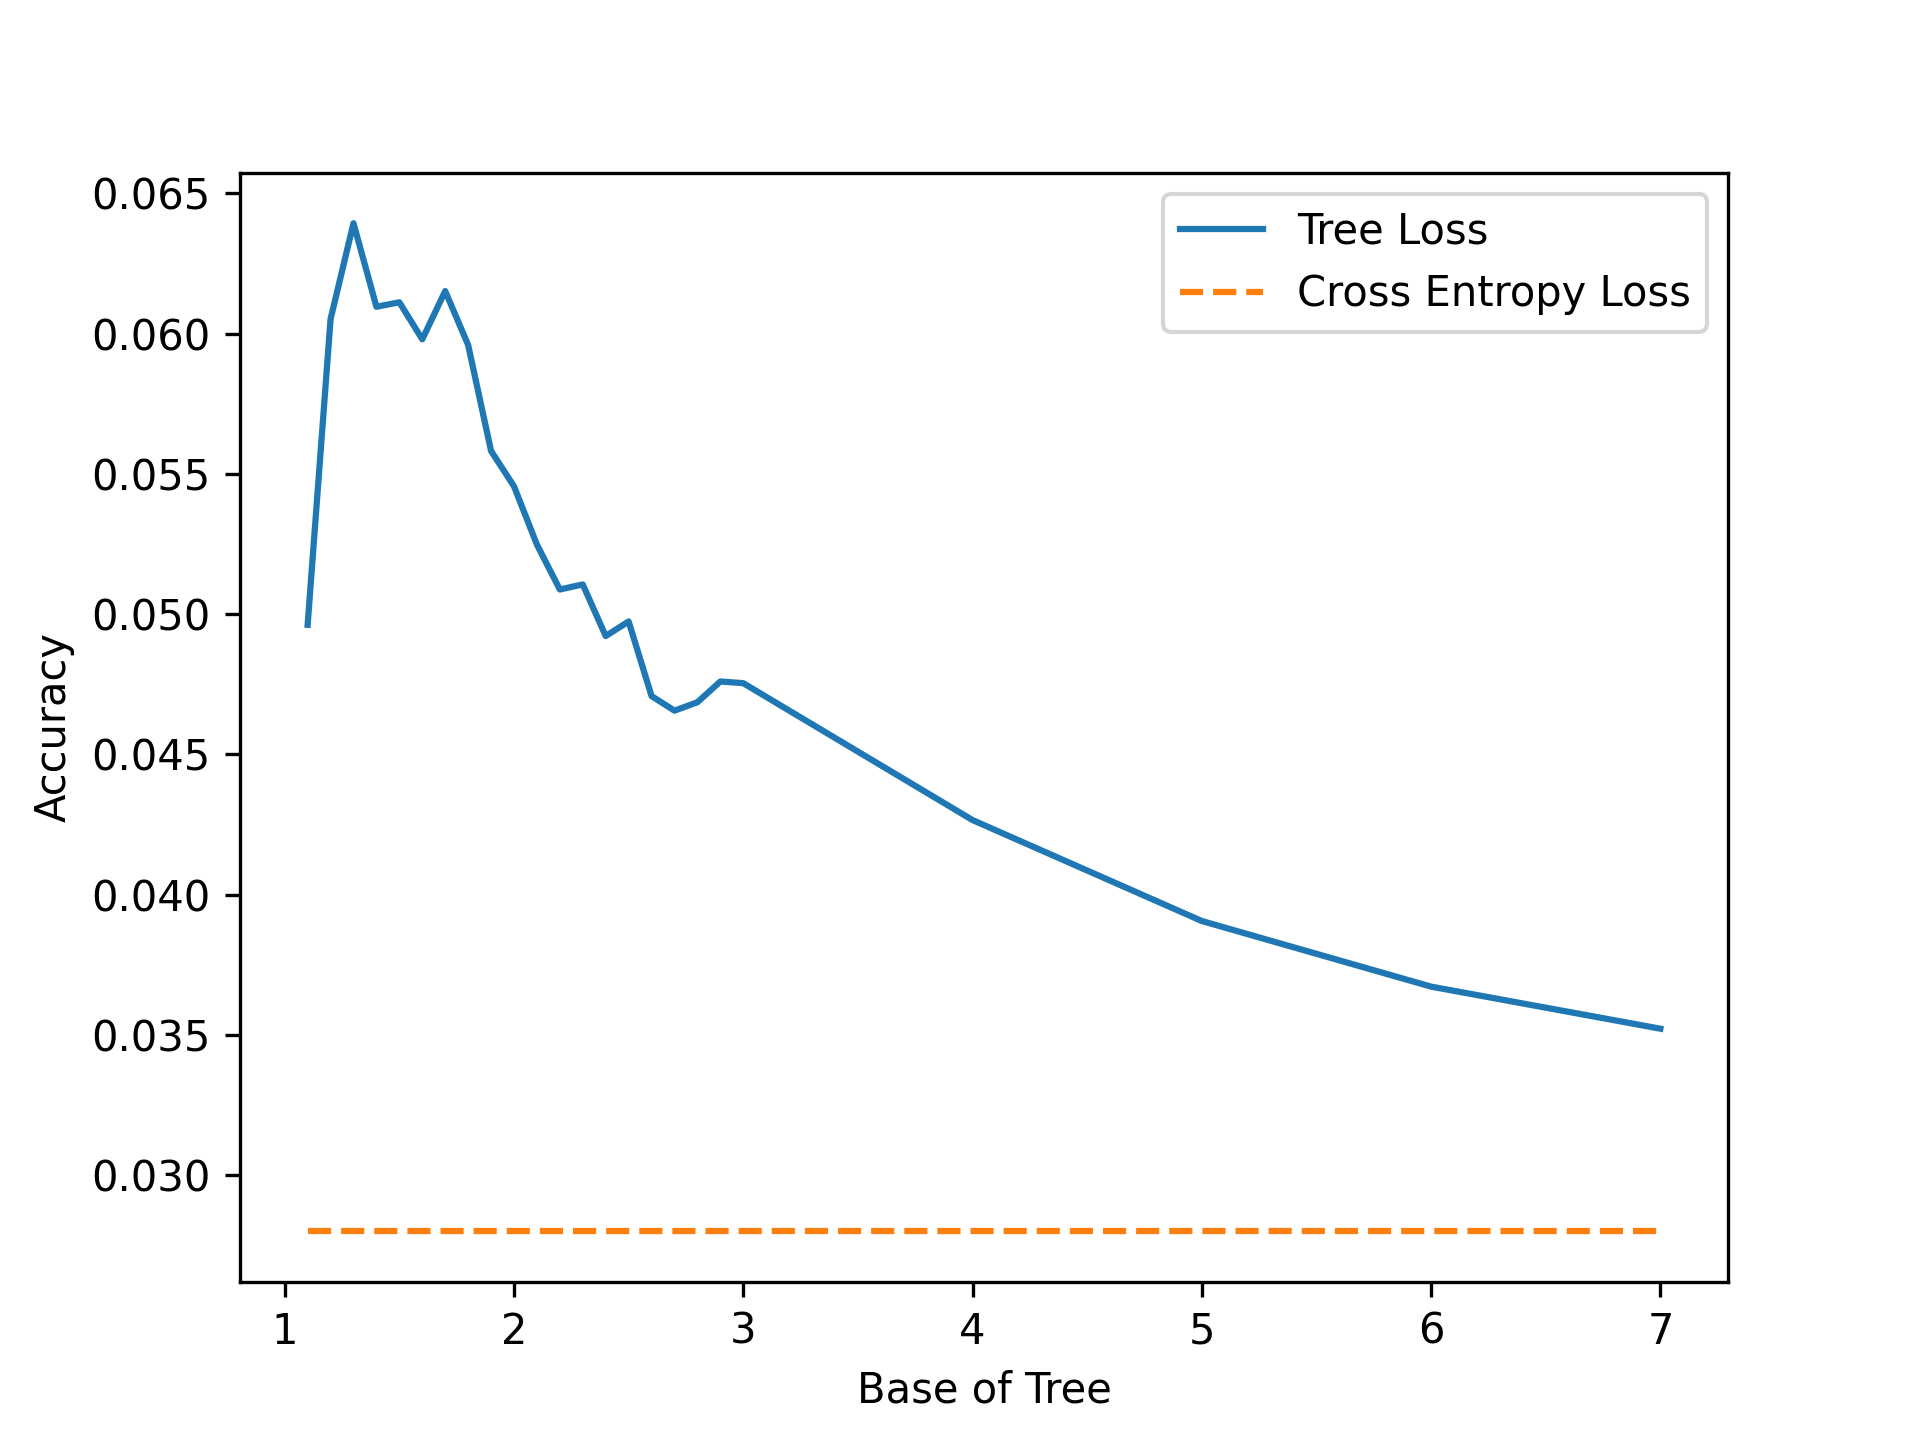
\includegraphics[width=\columnwidth]{fig/new_img/accuracy_vs_base.png}
%\end{frame}

%%%%%%%%%%%%%%%%%%%%%%%%%%%%%%%%%%%%%%%%%%%%%%%%%%%%%%%%%%%%%%%%%%%%%%%%%%%%%%%%

\begin{frame}{Experiments: Synthetic: Bad Tree Structures}

Data generated as before.
Metric generated as:
\begin{align*}
    W^{\text{bad}}  &\sim \mathcal N(0,1)^{k\times d} \\
    d_\epsilon(i,j) &= \ltwo{(1-\epsilon)(\w_i^*-\w_j^*) + \epsilon(\w^{\text{bad}}_i - \w^{\text{bad}}_j)}
%\vspace{-0.1in}
\end{align*}
$\epsilon=0$ $\Rightarrow$ perfectly good metric

$\epsilon=1$ $\Rightarrow$ perfectly bad metric

    \vspace{-0.1in}
\begin{center}
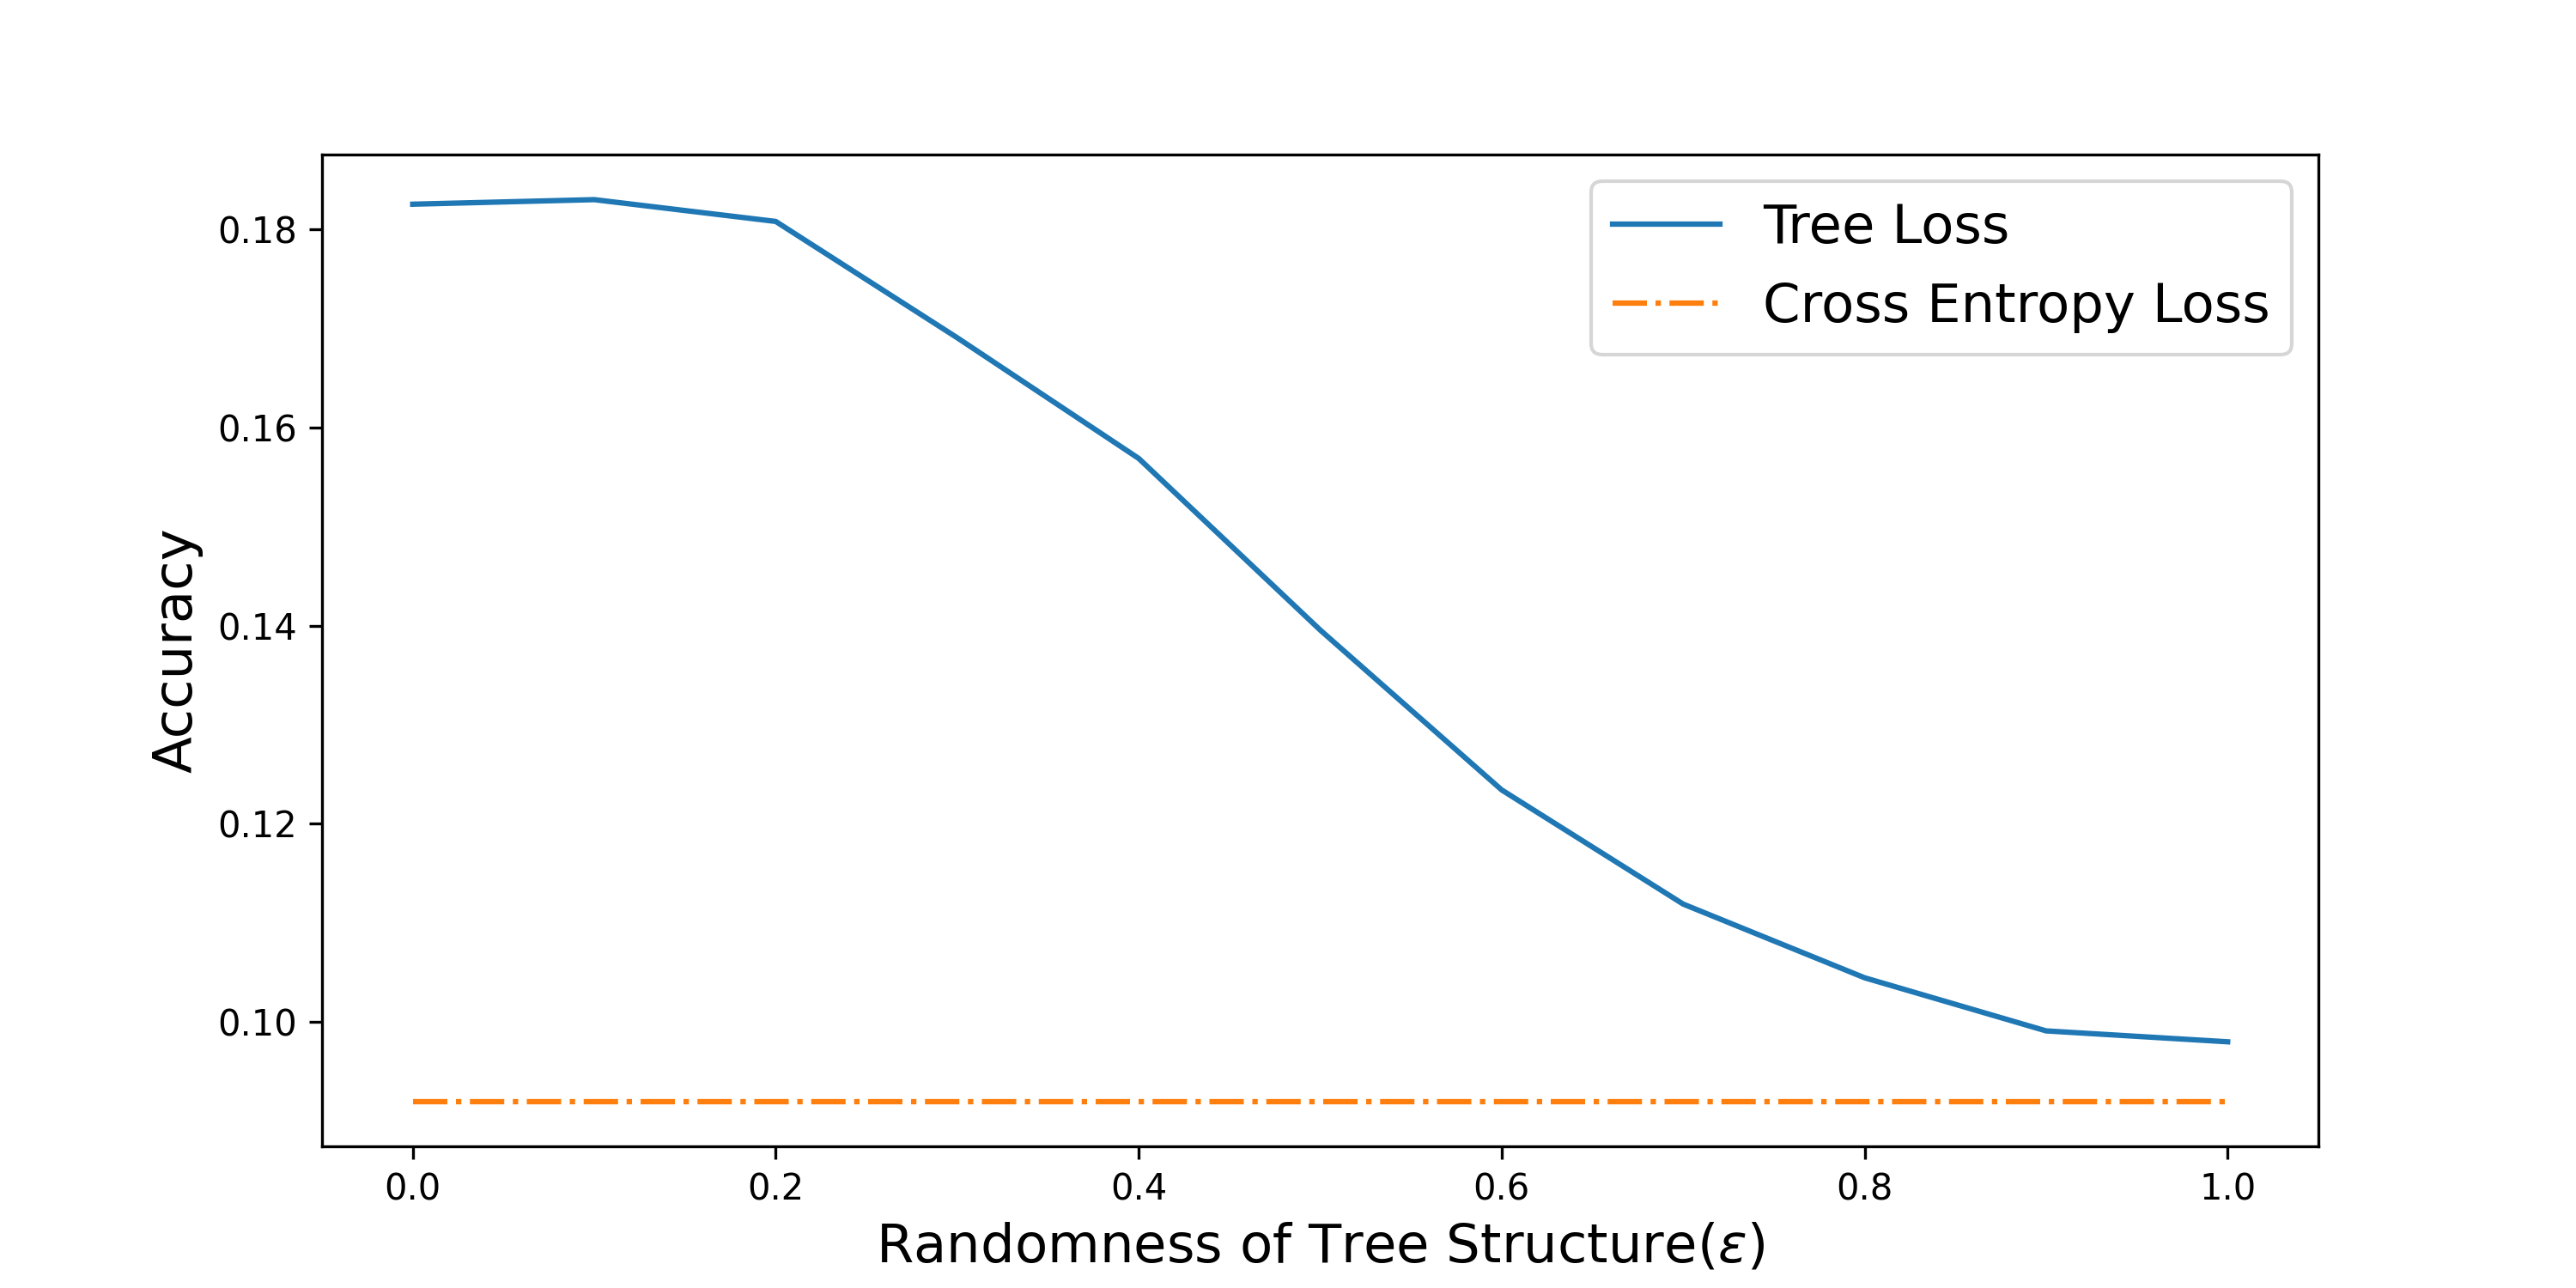
\includegraphics[width=0.8\columnwidth]{fig/new_img/loss_vs_structure.png}
\end{center}
\end{frame}
